\noindent In der Serienfertigung und der automatisierten Messtechnik entsteht eine Vielzahl von Daten. Die Datens\"{a}tze sind oft komplex und un\"{u}bersichtlich, eine Interpretation aller Daten im Detail ist zudem zeitaufw\"{a}ndig. Vor diesem Hintergrund ist es erforderlich, die Daten \"{u}bersichtlich darstellen oder auf Kenngr\"{o}{\ss}en komprimieren zu k\"{o}nnen.\newline

\noindent Als Einstieg in die Statistik besch\"{a}ftigt sich dieses Kapitel deshalb mit der Frage, wie Daten numerisch und grafisch aufbereitet werden k\"{o}nnen. Anschlie{\ss}end wird die zusammenfassende Beschreibung von Datens\"{a}tzen mit Hilfe statistischer Kenngr\"{o}{\ss}en eingef\"{u}hrt. 

\subsection{ Merkmalstypen}

\noindent Der Design For Six Sigma (DFSS) Prozess zeichnet sich dadurch aus, dass \"{u}ber den gesamten Prozess quantitative Methoden eingesetzt werden. Die Ergebnisse sind dabei von definierten Merkmalen abh\"{a}ngig. Die Merkmale k\"{o}nnen unterschiedlicher Natur sein. Vor dem Einsatz statistischer Methoden ist es notwendig, die unterschiedlichen Merkmalstypen zu klassifizieren, da sie einen Einfluss auf die Methodik und die Genauigkeit der Aussage haben. Die f\"{u}r den Design For Six Sigma Prozess relevanten Merkmalstypen lassen sich in stetige und diskrete Gr\"{o}{\ss}en, sowie ordinale und gruppierende Gr\"{o}{\ss}en aufteilen. 

\subsubsection{Stetige Merkmale}

\noindent Stetige Merkmale k\"{o}nnen eine Eigenschaft beliebig fein wiedergeben. Es entsteht kein Fehler durch die Darstellung des Ergebnisses, allenfalls durch die Aufzeichnung des Messergebnisses. Beispiele f\"{u}r stetige Merkmale sind Temperaturen, elektrische Spannungen und Str\"{o}me, geometrische Ma{\ss}e wie Strecken oder Fl\"{a}cheninhalte sowie die Zeit. Stetige Merkmale werden bei einer Verarbeitung der Werte im Rechner diskretisiert. Sind die Stufen der Diskretisierung eine Gr\"{o}{\ss}enordnung kleiner als die kleinste darzustellende Gr\"{o}{\ss}e, kann die Quantisierung vernachl\"{a}ssigt werden. Die Merkmale werden als quasi-stetig bezeichnet.


\subsubsection{Diskrete Merkmale}

\noindent Diskrete Merkmale haben nur endlich viele Auspr\"{a}gungen. Zum Beispiel kann ein Wurf mit einem W\"{u}rfel nur die Zahlen eins bis sechs annehmen, und er weist nur endlich viele unterschiedliche Ereignisse auf. Eine Erfassung von stetigen Gr\"{o}{\ss}en mit diskreten Messmitteln f\"{u}hrt zu einer diskreten Messgr\"{o}{\ss}e. Beispielsweise f\"{u}hrt die Messung einer Spannung mit einem 6 Bit Analog-Digital-Wandler und einem Messbereich von 5 V zu einem Quantisierungsintervall von 

\begin{equation}\label{eq:threeone}
\Delta U=\dfrac{5 V}{2^{6} } =78 mV
\end{equation}

\noindent Ist diese Diskretisierung gr\"{o}{\ss}er als ein Zehntel der interessierenden kleinsten Spannung, wird das urspr\"{u}nglich stetige Merkmal als diskretes Merkmal bezeichnet. \newline

\noindent Ein diskretes Merkmal entsteht auch bei der Klassenbildung von stetigen Merkmalen. Zum Beispiel ist es denkbar, die Rohwerte einer Widerstandsmessung in Klassen zusammenzufassen, die einem Widerstandsbereich entsprechen. Nach der Klassenbildung kann nicht mehr entschieden werden, ob der Widerstand am unteren oder oberen Ende des Intervalls lag. Aus dem stetigen Merkmal ist durch die Klassenbildung ein diskretes Merkmal entstanden.

\subsubsection{Ordinale Merkmale}

\noindent Ordinale Datentypen werden f\"{u}r Daten verwendet, die nach ihrer Auspr\"{a}gung geordnet werden k\"{o}nnen, deren Abst\"{a}nde aber nicht interpretiert werden k\"{o}nnen. Ein typisches Beispiel daf\"{u}r sind Kontrollergebnisse, die zu einer Aussage ,,gut``, ,,m\"{a}{\ss}ig`` oder ,,schlecht`` f\"{u}hren. Diese Aussage kann in Zahlen wiedergegeben werden, zum Beispiel kann der Eigenschaft ,,gut`` die Zahl 1, ,,m\"{a}{\ss}ig`` die Zahl 2 und ,,schlecht`` die Zahl 3 zugeordnet werden. Diese Zuordnung gibt jedoch nur ein Ordnungsschema an. Im Gegensatz zu den stetigen und diskreten Datentypen kann mit ordinalen Datentypen nicht sinnvoll gerechnet werden, vielleicht mit Ausnahme der Fuzzy Logik. Au{\ss}erdem sind die Aussagen ,,gut``, ,,m\"{a}{\ss}ig`` oder ,,schlecht`` deutlich gr\"{o}ber und schlechter zu interpretieren als numerische Angaben mit stetigen oder diskreten Daten.


\subsubsection{Gruppierende Merkmale}

\noindent Gruppierende Merkmale sind zum Beispiel bei der Charakterisierung von Verfahren zu finden. Wird ein Verfahren ge\"{a}ndert, erfolgt ein Vergleich des alten Verfahrens mit dem neuen. Auch Zulieferer lassen sich nicht ordnen, sie existieren parallel und k\"{o}nnen nicht nach einer Auspr\"{a}gung geordnet werden. Gruppierende Merkmale werden deshalb im Allgemeinen auch nicht mit Zahlen bezeichnet. 


\subsubsection{Merkmalstypen und Aussagesicherheit}

\noindent Aus der Beschreibung der unterschiedlichen Merkmalstypen ergibt sich, dass die Genauigkeit bei Messungen von stetigen Merkmalen zu gruppierenden Merkmalen kontinuierlich abnimmt. Ordinalen und gruppierenden Datentypen kann eine mathematisch berechnete Kenngr\"{o}{\ss}e nicht mehr sinnvoll zugeordnet werden. Aus diesem Grund unterscheiden sich auch die statistischen Methoden, die f\"{u}r die stetigen und diskreten Datentypen eingesetzt werden, von denen, die f\"{u}r die ordinalen und gruppierten Datentypen verwendet werden. 

\noindent Der Schwerpunkt liegt in den folgenden Kapiteln auf stetigen und diskreten Datentypen, die nur von einer Einflussgr\"{o}{\ss}e abh\"{a}ngen. 

\clearpage

\subsection{H\"{a}ufigkeitsverteilungen}

\noindent Statistische Daten werden durch Aufzeichnen von Beobachtungsergebnissen gewonnen. Die dabei entstehende Liste wird als Urliste bezeichnet. Tabelle \ref{tab:threeone} stellt die Messwerte von N = 100 Widerst\"{a}nden mit einem Sollwert von $R = 1 k\Omega$ dar. Die Daten weisen eine Aufl\"{o}sung von $\Delta R = 1 \Omega$ auf. Es handelt sich deshalb um einen diskreten Merkmalstyp.

\begin{table}[H]
\setlength{\arrayrulewidth}{.1em}
\caption{Beispiel f\"{u}r eine Urliste: Messwerte von 100 Widerst\"{a}nden mit einem Sollwert von $R = 1 k \Omega $}
\setlength{\fboxsep}{0pt}%
\colorbox{lightgray}{%
\arrayrulecolor{white}%
\begin{tabular}{| wc{2cm} | wc{1cm} | wc{1cm} | wc{1cm} | wc{1cm} | wc{1cm} | wc{1cm} | wc{1cm} | wc{1cm} | wc{1cm} | wc{1cm} }
\hline\xrowht{15pt}

\fontfamily{phv}\selectfont\textbf{Index} & \multicolumn{10}{c}{\fontfamily{phv}\selectfont\textbf{Messwert R / $\Omega$}} \\ \hline \xrowht{15pt}

\fontfamily{phv}\selectfont\textbf{1 - 10} &
983 & 988 & 985 & 987 & 988 & 987 & 986 & 985 & 986 & 991\\ \hline\xrowht{15pt}

\fontfamily{phv}\selectfont\textbf{11 - 20} & 
987 & 986 & 987 & 986 & 985 & 988 & 986 & 986 & 988 & 985\\ \hline\xrowht{15pt}

\fontfamily{phv}\selectfont\textbf{21 - 30} &
985 & 989 & 986 & 986 & 985 & 992 & 988 & 989 & 986 & 986\\ \hline\xrowht{15pt}

\fontfamily{phv}\selectfont\textbf{31 - 40} &
985 & 986 & 986 & 986 & 989 & 988 & 986 & 986 & 986 & 987\\ \hline\xrowht{15pt}

\fontfamily{phv}\selectfont\textbf{41 - 50} &
989 & 986 & 986 & 985 & 988 & 990 & 986 & 986 & 988 & 987\\ \hline\xrowht{15pt}

\fontfamily{phv}\selectfont\textbf{51 - 60} &
985 & 989 & 987 & 985 & 986 & 990 & 986 & 985 & 986 & 988\\ \hline\xrowht{15pt}

\fontfamily{phv}\selectfont\textbf{61 - 70} &
985 & 988 & 984 & 988 & 986 & 985 & 987 & 989 & 986 & 987\\ \hline\xrowht{15pt}

\fontfamily{phv}\selectfont\textbf{71 - 80} &
987 & 987 & 985 & 987 & 986 & 986 & 986 & 987 & 985 & 989\\ \hline\xrowht{15pt}

\fontfamily{phv}\selectfont\textbf{81 - 90} &
988 & 992 & 985 & 986 & 987 & 987 & 985 & 988 & 984 & 988\\ \hline\xrowht{15pt}

\fontfamily{phv}\selectfont\textbf{91 - 100} &
987 & 988 & 985 & 986 & 986 & 985 & 987 & 989 & 986 & 985\\ \hline
\end{tabular}%
}
\label{tab:threeone}
\end{table}

\noindent Die in Tabelle \ref{tab:threeone} dargestellten Gr\"{o}{\ss}en bilden eine Stichprobe mit dem Umfang N = 100, die einzelnen Messwerte werden allgemein als Stichprobenwerte bezeichnet. Mithilfe der Wahrscheinlichkeitsrechnung wird sp\"{a}ter versucht, von der Stichprobe auf die Grundgesamtheit, zum Beispiel aller Widerst\"{a}nde in einem definierten Fertigungszeitraum, zu schlie{\ss}en. \newline

\noindent Zur \"{U}bersicht k\"{o}nnen die Daten in einem sogenannten Streudiagramm dargestellt werden. Dabei wird der Stichprobenindex als Abszisse und der Stichprobenwert als Ordinate dargestellt. 

\noindent 
\begin{figure}[H]
  \centerline{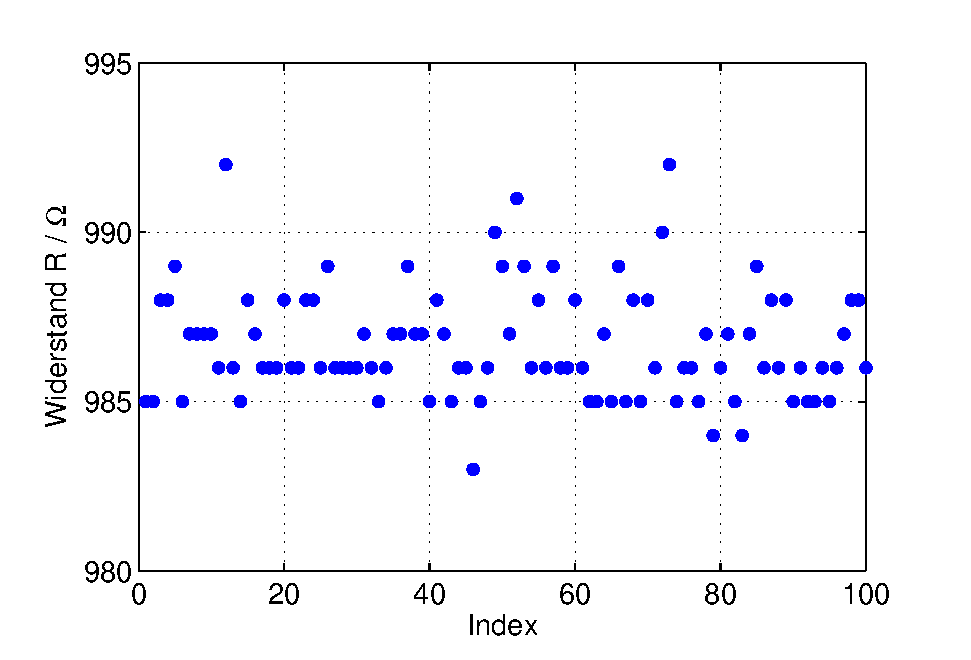
\includegraphics[width=0.5\textwidth]{Kapitel3/Bilder/image1}}
  \caption{Darstellung der Stichprobe in Tabelle \ref{tab:threeone} als Streudiagramm}
  \label{fig:RelHaeufigkeitUndSummenhStichprobeWiderstand1}
\end{figure}

\subsubsection{Absolute und relative H\"{a}ufigkeit diskreter Merkmalstypen}\label{threetwoone}

\noindent Zur \"{u}bersichtlichen Darstellung der Stichprobenwerte diskreter Merkmalstypen werden die Stichproben der Gr\"{o}{\ss}e nach geordnet, und die H\"{a}ufigkeit der einzelnen Werte wird ausgewertet. Bei manueller Ausf\"{u}hrung ergibt sich zun\"{a}chst eine Strichliste wie in Tabelle \ref{tab:threetwo}, aus der anschlie{\ss}end eine H\"{a}ufigkeitsverteilung wie in Tabelle 3.3 abgeleitet werden kann.


\begin{table}[H]
\caption{H\"{a}ufigkeitsbewertung \"{u}ber eine Strichliste }
\setlength{\fboxsep}{0pt}%
\colorbox{lightgray}{%
\arrayrulecolor{white}%
\begin{tabular}{| c | c | c | c |}
\hline
\parbox[c][0.28in][c]{1in}{\smallskip\centering\textbf{\fontfamily{phv}\selectfont{R / $\mathbf{\Omega}$}}} & 
\parbox[c][0.28in][c]{2.1in}{\smallskip\centering\textbf{\fontfamily{phv}\selectfont{Absolute H\"{a}ufigkeit h$_{\mathbf{A}}$(R)}}} &
\parbox[c][0.28in][c]{1in}{\smallskip\centering\textbf{\fontfamily{phv}\selectfont{R / $\mathbf{\Omega}$}}} &
\parbox[c][0.28in][c]{2.1in}{\smallskip\centering\textbf{\fontfamily{phv}\selectfont{Absolute H\"{a}ufigkeit h$_{\mathbf{A}}$(R)}}}\\ \hline

\parbox[c][0.28in][c]{1in}{\centering\fontfamily{phv}\selectfont{983}} &
\parbox[c][0.28in][c]{2.1in}{\centering{I}} &
\parbox[c][0.28in][c]{1in}{\centering\fontfamily{phv}\selectfont{988}} &
\parbox[c][0.28in][c]{2.1in}{\centering{IIII IIII IIII}} \\ \hline

\parbox[c][0.28in][c]{1in}{\centering\fontfamily{phv}\selectfont{984}} &
\parbox[c][0.28in][c]{2.1in}{\centering{II}} &
\parbox[c][0.28in][c]{1in}{\centering\fontfamily{phv}\selectfont{989}} &
\parbox[c][0.28in][c]{2.1in}{\centering{IIII III}} \\ \hline

\parbox[c][0.28in][c]{1in}{\centering\fontfamily{phv}\selectfont{985}} &
\parbox[c][0.28in][c]{2.1in}{\centering{IIII IIII IIII IIII}} &
\parbox[c][0.28in][c]{1in}{\centering\fontfamily{phv}\selectfont{990}} &
\parbox[c][0.28in][c]{2.1in}{\centering{II}} \\ \hline

\parbox[c][0.28in][c]{1in}{\centering\fontfamily{phv}\selectfont{986}} &
\parbox[c][0.28in][c]{2.1in}{\centering{IIII IIII IIII IIII IIII IIII II}} &
\parbox[c][0.28in][c]{1in}{\centering\fontfamily{phv}\selectfont{991}} &
\parbox[c][0.28in][c]{2.1in}{\centering{I}} \\ \hline

\parbox[c][0.28in][c]{1in}{\centering\fontfamily{phv}\selectfont{987}} &
\parbox[c][0.28in][c]{2.1in}{\centering{IIII IIII IIII II}} &
\parbox[c][0.28in][c]{1in}{\centering\fontfamily{phv}\selectfont{992}} &
\parbox[c][0.28in][c]{2.1in}{\centering{II}} \\ \hline

\end{tabular}%
}\bigskip
\label{tab:threetwo}
\end{table}

\begin{table}[H]
\caption{Häufigkeitsverteilung der Stichprobe}
\setlength{\fboxsep}{0pt}%
\colorbox{lightgray}{%
\arrayrulecolor{white}%
\begin{tabular}{| c | c | c | c | c | c |}
\hline
\parbox[c][0.7in][c]{0.97in}{\smallskip\centering\textbf{\fontfamily{phv}\selectfont{R / $\mathbf{\Omega}$}}} & 
\parbox[c][0.7in][c]{0.97in}{\smallskip\centering\textbf{\fontfamily{phv}\selectfont{Absolute\\ H\"{a}ufigkeit\\ h$_{\mathbf{A}}$(R)}}} &
\parbox[c][0.7in][c]{0.97in}{\smallskip\centering\textbf{\fontfamily{phv}\selectfont{Relative\\ H\"{a}ufigkeit\\ h$_{\mathbf{A}}$(R)}}} &
\parbox[c][0.7in][c]{0.97in}{\smallskip\centering\textbf{\fontfamily{phv}\selectfont{R / $\mathbf{\Omega}$}}} &
\parbox[c][0.7in][c]{0.97in}{\smallskip\centering\textbf{\fontfamily{phv}\selectfont{Absolute\\ H\"{a}ufigkeit\\ h$_{\mathbf{A}}$(R)}}} &
\parbox[c][0.7in][c]{0.97in}{\smallskip\centering\textbf{\fontfamily{phv}\selectfont{Relative\\ H\"{a}ufigkeit\\ h$_{\mathbf{A}}$(R)}}}\\ \hline

\parbox[c][0.28in][c]{0.97in}{\centering{983}} &
\parbox[c][0.28in][c]{0.97in}{\centering{1}} &
\parbox[c][0.28in][c]{0.97in}{\centering{0.01}} &
\parbox[c][0.28in][c]{0.97in}{\centering{988}} &
\parbox[c][0.28in][c]{0.97in}{\centering{15}} &
\parbox[c][0.28in][c]{0.97in}{\centering{0.15}} \\ \hline

\parbox[c][0.28in][c]{0.97in}{\centering{984}} &
\parbox[c][0.28in][c]{0.97in}{\centering{2}} &
\parbox[c][0.28in][c]{0.97in}{\centering{0.02}} &
\parbox[c][0.28in][c]{0.97in}{\centering{989}} &
\parbox[c][0.28in][c]{0.97in}{\centering{8}} &
\parbox[c][0.28in][c]{0.97in}{\centering{0.08}} \\ \hline

\parbox[c][0.28in][c]{0.97in}{\centering{985}} &
\parbox[c][0.28in][c]{0.97in}{\centering{20}} &
\parbox[c][0.28in][c]{0.97in}{\centering{0.20}} &
\parbox[c][0.28in][c]{0.97in}{\centering{990}} &
\parbox[c][0.28in][c]{0.97in}{\centering{2}} &
\parbox[c][0.28in][c]{0.97in}{\centering{0.02}} \\ \hline

\parbox[c][0.28in][c]{0.97in}{\centering{986}} &
\parbox[c][0.28in][c]{0.97in}{\centering{32}} &
\parbox[c][0.28in][c]{0.97in}{\centering{0.32}} &
\parbox[c][0.28in][c]{0.97in}{\centering{991}} &
\parbox[c][0.28in][c]{0.97in}{\centering{1}} &
\parbox[c][0.28in][c]{0.97in}{\centering{0.01}} \\ \hline

\parbox[c][0.28in][c]{0.97in}{\centering{987}} &
\parbox[c][0.28in][c]{0.97in}{\centering{17}} &
\parbox[c][0.28in][c]{0.97in}{\centering{0.17}} &
\parbox[c][0.28in][c]{0.97in}{\centering{992}} &
\parbox[c][0.28in][c]{0.97in}{\centering{2}} &
\parbox[c][0.28in][c]{0.97in}{\centering{0.02}} \\ \hline

\end{tabular}%
}\bigskip
\label{tab:threethree}
\end{table}

\noindent Die absolute H\"{a}ufigkeit gibt an, wie oft der entsprechende Messwert x in der Stichprobe die Auspr\"{a}gung $x{}_{n}$ annimmt. Diese Anzahl wird als absolute H\"{a}ufigkeit $h{}_{A}(x)$ bezeichnet. Die relative H\"{a}ufigkeit $h(x)$ ergibt sich aus dem Quotient aus absoluter H\"{a}ufigkeit $h{}_{A}$(x) und dem Stichprobenumfang~N.

\begin{equation}\label{eq:threetwo}
h(x)=\dfrac{h_{A} (x)}{N} 
\end{equation}

\noindent Zum Beispiel kommt die Auspr\"{a}gung mit einem Widerstandswert von $R = 988 \Omega$ in der Stichprobe 15-mal vor. Da die Stichprobe insgesamt $N = 100$ Werte aufweist, ergibt sich eine relative H\"{a}ufigkeit von $15 \%$.

\noindent Kommt der Wert $x_{0}$ in der Stichprobe nicht vor, hat er die absolute H\"{a}ufigkeit $h_{A}(x_{0})$ = 0 und nach Gleichung \eqref{eq:twothirtyseven} auch die relative H\"{a}ufigkeit $h(x_{0}) = 0$. Im anderen Extremfall k\"{o}nnten alle Stichprobenwerte die Auspr\"{a}gung $x_{1}$ haben. In diesem Fall w\"{a}re die absolute H\"{a}ufigkeit $h_{A}(x_{1}) = N$ und damit die relative H\"{a}ufigkeit $h(x_{1}) = 1$. Die relative H\"{a}ufigkeit $h(x)$ ist somit eine nicht negative Zahl, die h\"{o}chstens den Wert 1 annehmen kann.

\begin{equation}\label{eq:threethree}
0\le h(x)\le 1
\end{equation}

\noindent Die Zahlenwerte in Tabelle \ref{tab:threethree} stellen die H\"{a}ufigkeitsverteilung h(x) der Stichprobe dar. Sie ordnet jedem Wert x eine relative H\"{a}ufigkeit h(x) zu. Die Summe aller absoluten H\"{a}ufigkeiten muss die Anzahl von Stichprobenwerten N ergeben. Die Summe aller relativen H\"{a}ufigkeiten ist damit 1. Es gilt: 

\begin{equation}\label{eq:threefour}
h(x_{1})+h(x_{2} )+h)+{\rm \; ...\; }+h(x_{N})=\sum _{n=1}^{N}h(x_{n} )=1
\end{equation}

\noindent Zur besseren \"{U}bersicht k\"{o}nnen die absolute oder die relative H\"{a}ufigkeit in Form von Stab- oder Liniendiagrammen dargestellt werden. Bild \ref{fig:HaeufigkeitStichprobeWiderstand} stellt die relative H\"{a}ufigkeit f\"{u}r die Stichprobe in Tabelle \ref{tab:threeone} als Histogramm dar.

\noindent 
\begin{figure}[H]
  \centerline{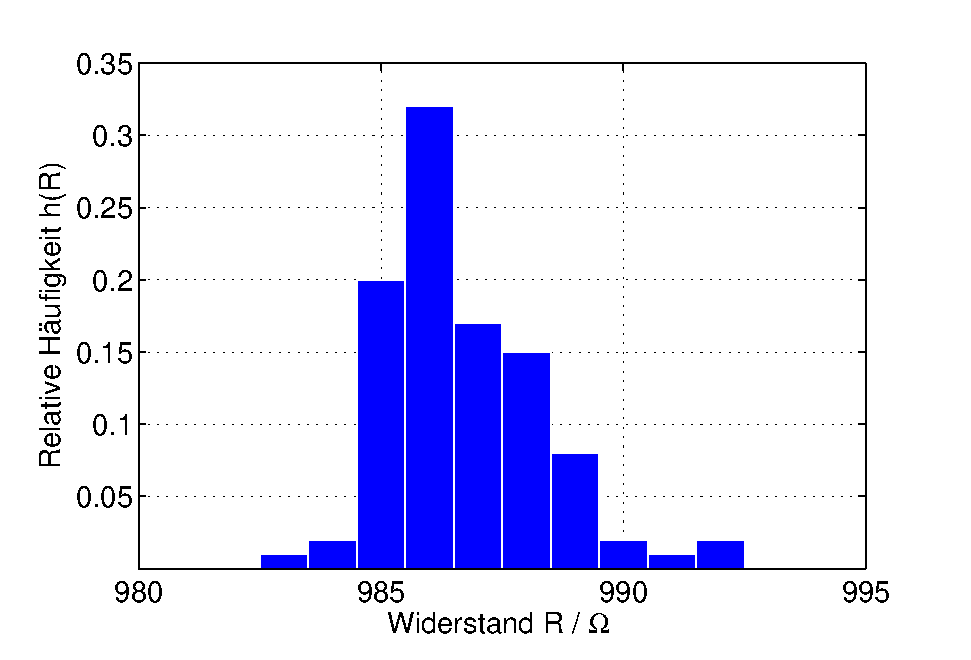
\includegraphics[width=0.5\textwidth]{Kapitel3/Bilder/image2}}
  \caption{Darstellung der relativen H\"{a}ufigkeiten als Stabdiagramm f\"{u}r die Stichprobe in Tabelle \ref{tab:threeone}}
  \label{fig:HaeufigkeitStichprobeWiderstand}
\end{figure}

\noindent Bei sehr vielen unterschiedlichen Zahlenwerten der Stichprobe wird die H\"{a}ufigkeitsverteilung un\"{u}bersichtlich. Aus diesem Grund k\"{o}nnen die Stichprobenwerte in Klassen eingeteilt werden. Ausgehend von dem Gesamtintervall, in dem die Stichprobenwerte liegen, werden Teilintervalle oder Klassenintervalle gebildet. Die Mittenwerte $c_{n}$ der Intervalle hei{\ss}en Klassenmitten. Die einzelnen Stichprobenwerte werden den entsprechenden Teilintervallen oder Klassen zugeordnet. Es ergibt sich die absolute und analog zu Gleichung \eqref{eq:threetwo} die relative Klassenh\"{a}ufigkeit. Die H\"{a}ufigkeit in Abh\"{a}ngigkeit der Klassenmitten hei{\ss}t H\"{a}ufigkeitsverteilung der in Klassen eingeteilten Stichprobe.\newline

\noindent Nach der Aufteilung in Klassen treten die urspr\"{u}nglichen Stichprobenwerte nicht mehr einzeln in Erscheinung, sie gehen nur als Summe in die H\"{a}ufigkeitsverteilung der in Klassen eingeteilten Stichprobe ein. Je weniger Klassen gebildet werden, desto mehr Information geht verloren. Eine ungeeignete Anzahl oder Einteilung von Klassen f\"{u}hrt zu un\"{u}bersichtlichen oder falschen Interpretationsergebnissen. Bei der Definition von Stichprobenklassen haben sich folgende Regeln als sinnvoll erwiesen:

\begin{itemize}
    \item  Die Klassenintervalle sind gleich gro{\ss} zu w\"{a}hlen.
    \item  Die Klassenmitten sollen m\"{o}glichst einfache Zahlen mit m\"{o}glichst wenigen Ziffern sein.
    \item  Die Anzahl von Klassen sollte zwischen 10 und 20 liegen, sinnvoll ist eine Anzahl von Klassen mit 
\end{itemize}

\begin{equation}\label{eq:threefive}
Anzahl\approx \sqrt{N}
\end{equation}

\noindent Werden die Widerstandswerte aus Tabelle \ref{tab:threeone} in drei oder sechs Klassen eingeteilt, ergibt sich die in Bild \ref{fig:HaeufigkeitStichprobeWiderstandKlassen} dargestellte relative H\"{a}ufigkeit.

\noindent 
\begin{figure}[H]
  \centerline{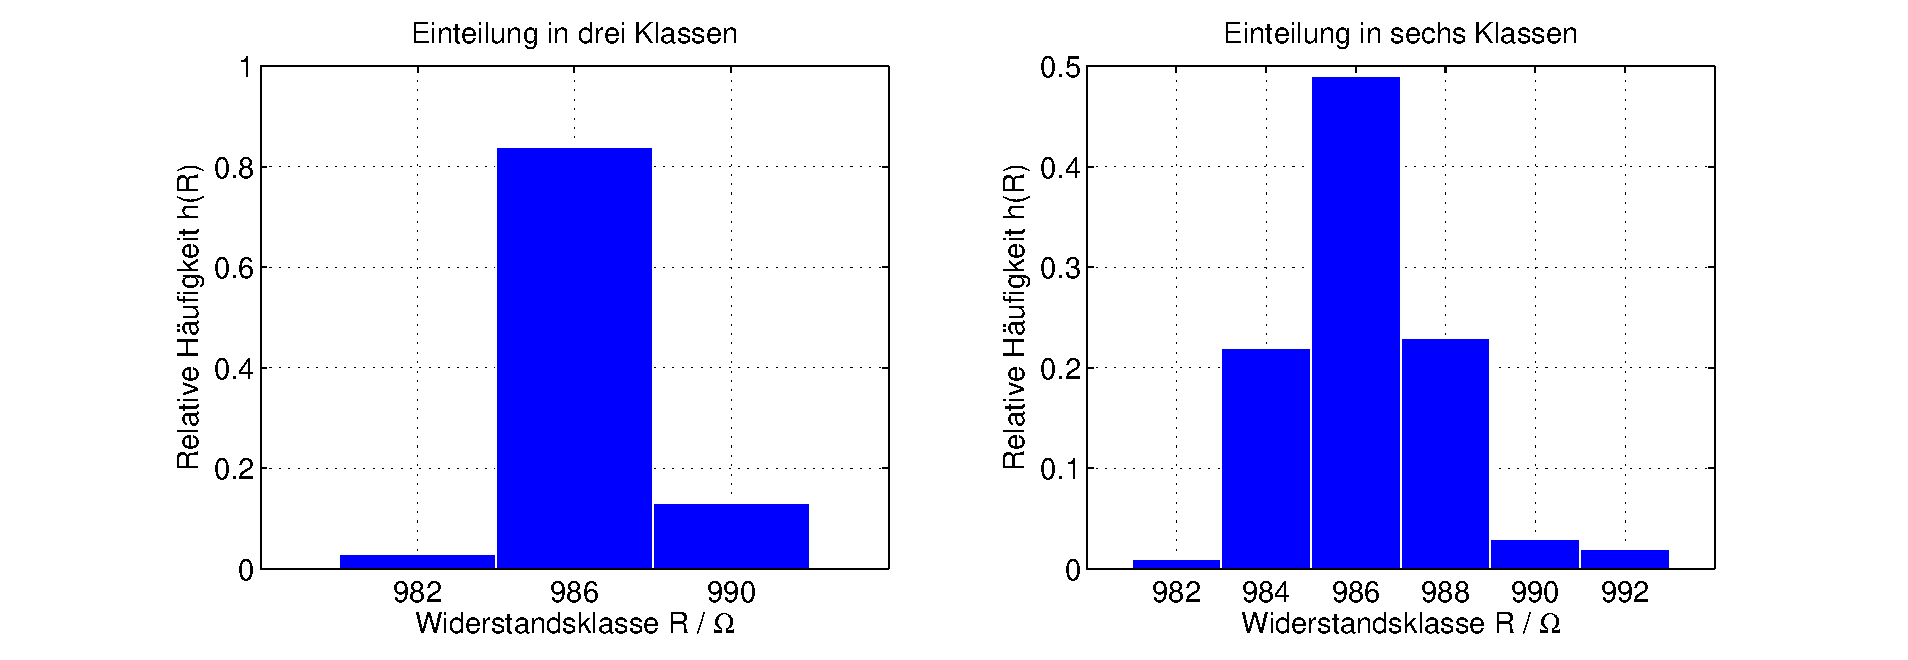
\includegraphics[width=1\textwidth]{Kapitel3/Bilder/image3}}
  \caption{Darstellung der relativen H\"{a}ufigkeiten f\"{u}r die Stichprobe in Tabelle \ref{tab:threeone}}
  \label{fig:HaeufigkeitStichprobeWiderstandKlassen}
\end{figure}

\noindent Dabei wird bei der Darstellung im Stabdiagramm das Prinzip der Fl\"{a}chentreue eingehalten. Es besagt, dass die Fl\"{a}chen direkt proportional zu den absoluten beziehungsweise relativen H\"{a}ufigkeiten sein m\"{u}ssen. Wird der Abstand zwischen zwei benachbarten Klassenmitten $c_{n}$ und $c_{n-1}$ als Breite d mit 

\begin{equation}\label{eq:threesix}
d=c_{n} -c_{n-1}
\end{equation}

\noindent bezeichnet, so muss die H\"{o}he $h_{n}$ im Stabdiagramm den Wert 

\begin{equation}\label{eq:threeseven}
h_{n} =\dfrac{h\left(x_{n} \right)}{d}
\end{equation}

\noindent aufweisen, damit die Fl\"{a}che proportional zur relativen H\"{a}ufigkeit wird

\begin{equation}\label{eq:threeeight}
A_{n} =h_{n} \cdot d=\dfrac{h(x_{n})}{d} \cdot d=h(x_{n})
\end{equation}

\subsubsection{Absolute und relative Summenh\"{a}ufigkeit diskreter Merkmalstypen}\label{threetwotwo}

\noindent Die H\"{a}ufigkeitsverteilung h(x) der Stichprobe gibt die relativen H\"{a}ufigkeiten an, mit der die einzelnen Zahlenwerte in der Stichprobe vorkommen. Oft stellt sich aber die Frage, wie viele Stichprobenwerte unter oder auf einem Grenzwert liegen. Soll zum Beispiel f\"{u}r das Beispiel aus Tabelle \ref{tab:threeone} die Frage beantwortet werden, wie viele Widerst\"{a}nde kleiner oder gleich 985 $\Omega$ sind, muss die Summe

\begin{equation}\label{eq:threenine}
h(R\le 985 \Omega) = h(R=983 \Omega )+h(R=984 \Omega)+h(R=985\Omega )=0.23
\end{equation}

\noindent ausgewertet werden. Wird diese Summe f\"{u}r beliebige Werte x durchgef\"{u}hrt, ergibt sich die relative Summenh\"{a}ufigkeit H(x) der Stichprobe. H(x) ist die Summe der relativen H\"{a}ufigkeiten aller Stichprobenwerte, die kleiner oder gleich dem Wert x sind.

\begin{equation}\label{eq:threeten}
H(x)=\sum _{x_{n} =-\infty }^{x}h(x_{n})
\end{equation}

\noindent Bild \ref{fig:RelHaeufigkeitUndSummenhStichprobeWiderstand2} stellt die relative H\"{a}ufigkeit h(R) und die relative Summenh\"{a}ufigkeit H(R) f\"{u}r das Beispiel aus Tabelle \ref{tab:threeone} als Stabdiagramm dar.

\noindent 
\begin{figure}[H]
  \centerline{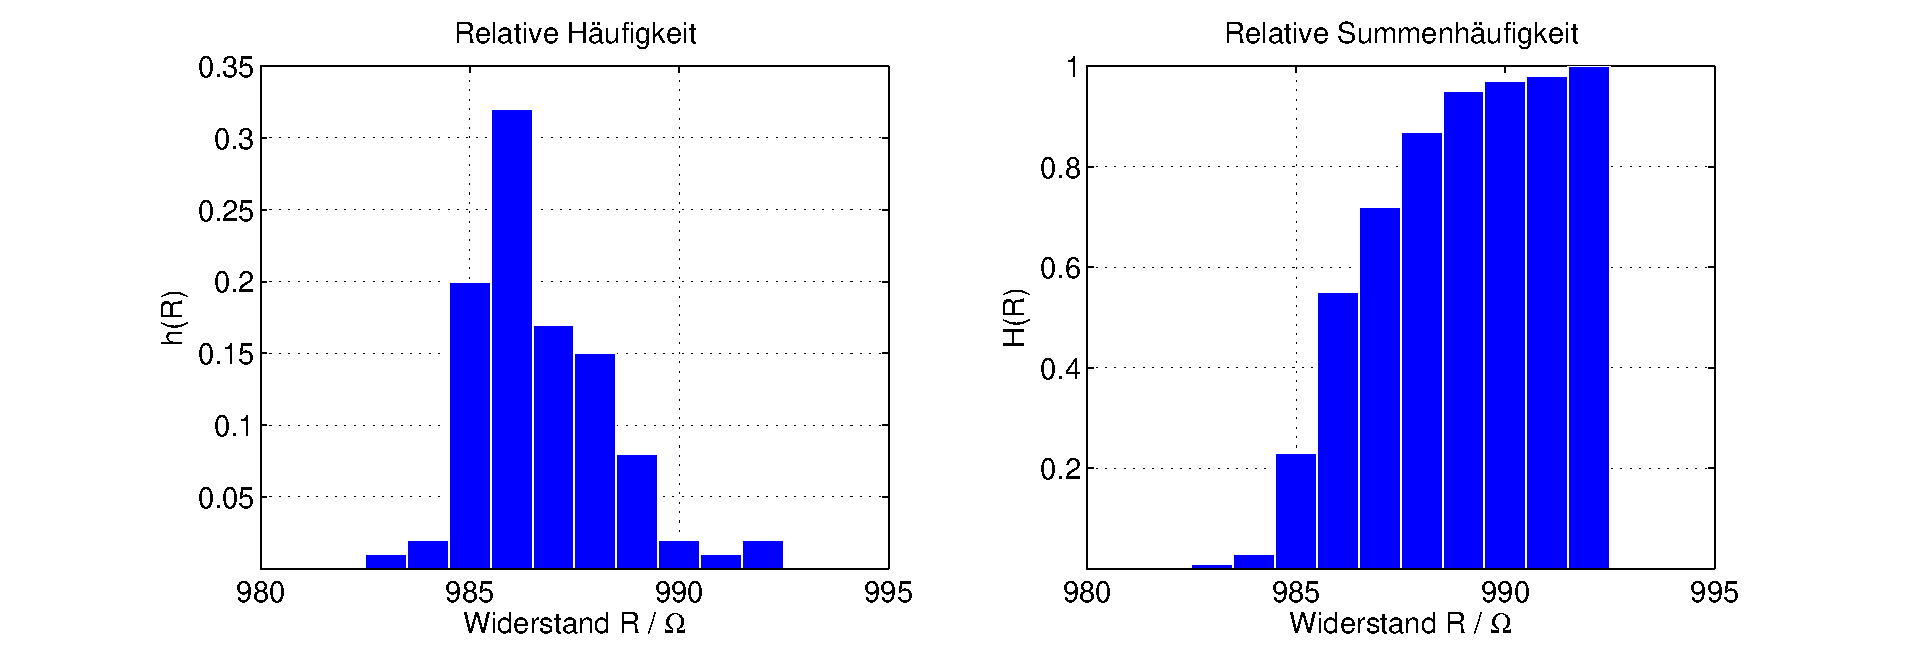
\includegraphics[width=1\textwidth]{Kapitel3/Bilder/image4}}
  \caption{Darstellung der relativen H\"{a}ufigkeit und Summenh\"{a}ufigkeit f\"{u}r die Stichprobe in Tabelle \ref{tab:threeone}}
  \label{fig:RelHaeufigkeitUndSummenhStichprobeWiderstand2}
\end{figure}

\noindent Die relative Summenh\"{a}ufigkeit erscheint zun\"{a}chst weniger anschaulich. In Abschnitt 3.2.3 wird sich aber zeigen, dass sie bei dem \"{U}bergang zu kontinuierlichen Stichprobenwerten einige Vorteile hat. Der Informationsgehalt ist bei der relativen H\"{a}ufigkeit und der relativen Summenh\"{a}ufigkeit identisch. Nach Gleichung \eqref{eq:threeten} kann die Summenh\"{a}ufigkeit aus der relativen H\"{a}ufigkeit berechnet werden.

\begin{equation}\label{eq:threeeleven}
H(x)=\sum _{x_{n} =-\infty }^{x}h(x_{n})
\end{equation}

\noindent Die Summenh\"{a}ufigkeit f\"{u}r den Wert (x -- d) ergibt sich entsprechend aus

\begin{equation}\label{eq:threetwelve}
H(x-d)=\sum _{x_{n} =-\infty }^{x-d}h(x_{n})
\end{equation}

\noindent Damit kann h(x) bestimmt werden aus der Differenz

\begin{equation}\label{eq:threethirteen}
h(x)=H(x)-H(x-d)
\end{equation}

\noindent Die Darstellungen k\"{o}nnen also mithilfe dieser Gleichungen ineinander \"{u}berf\"{u}hrt werden.

\subsubsection{Beschreibung stetiger Merkmalstypen}

\noindent Die anschauliche Beschreibung von Merkmalen mit einer relativen H\"{a}ufigkeit versagt bei stetigen Merkmalstypen, weil die Messwerte beliebig fein aufgel\"{o}st sind und jeder Messwert typischerweise nur einmal vorkommt. Liegen Stichproben mit stetigen Merkmalen vor, k\"{o}nnen die Werte gruppiert werden. Damit ergibt sich eine Auswertung, wie sie in den Abschnitten \ref{threetwoone} und \ref{threetwotwo} beschrieben ist. Allerdings gehen mit der Gruppierung der Merkmale Informationen verloren.\newline

\noindent Alternativ k\"{o}nnen stetige Merkmale mit einer relativen Summenh\"{a}ufigkeit beschrieben werden. Jeder Stichprobenwert einer Stichprobe mit stetigen Merkmalen kommt wegen der beliebig hohen Aufl\"{o}sung nur einmal vor. Bei einem Stichprobenumfang von N Werten weist jeder dieser Werte eine relative H\"{a}ufigkeit von 1/N auf. Alle anderen Werte weisen die relative H\"{a}ufigkeit von 0 auf. Durch Sortieren der Werte x nach der Gr\"{o}{\ss}e ergibt sich eine geordnete Stichprobe. Die relative Summenh\"{a}ufigkeit der Stichprobe ergibt sich aus 

\begin{equation}\label{eq:threefourteen}
H(x)=\sum _{x_{n} =-\infty }^{x}h(x_{n}) =\sum _{x_{n} =-\infty }^{x}\dfrac{1}{N}
\end{equation}

\noindent Je nach Werteverlauf der Stichprobe ergibt sich eine relative Summenh\"{a}ufigkeit, die grafisch als Liniendiagramm dargestellt werden kann. 

\noindent Bild \ref{fig:AuswertungDrucksensor} vergleicht die beiden Vorgehensweisen. Im linken Bildteil werden die Toleranzwerte einer Stichprobe mit N = 1000 Sensoren in Klassen eingeteilt und die relative Summenh\"{a}ufigkeit als Balkendiagramm dargestellt. Im rechten Bildteil ist die relative Summenh\"{a}ufigkeit ohne Gruppierung der Merkmale als Liniendiagramm eingezeichnet.

\noindent 
\begin{figure}[H]
  \centerline{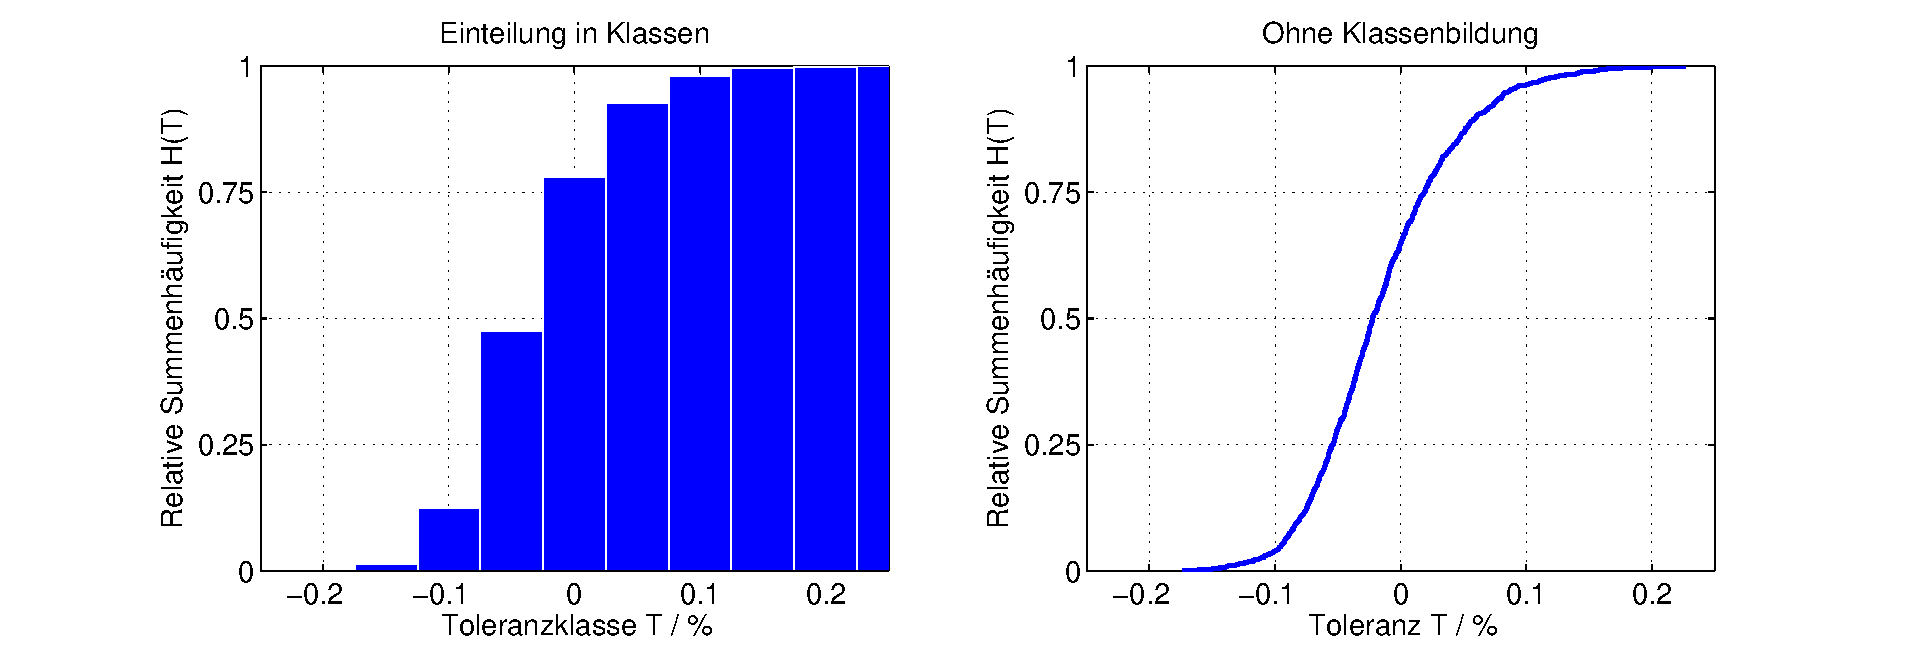
\includegraphics[width=1\textwidth]{Kapitel3/Bilder/image5}}
  \caption{Darstellung der Toleranzwerte eines Sensors}
  \label{fig:AuswertungDrucksensor}
\end{figure}

\noindent Anhand der Darstellung in Bild \ref{fig:AuswertungDrucksensor} wird unmittelbar deutlich, dass durch die Klassenbildung Information verloren gegangen ist, die Aufl\"{o}sung der Summenh\"{a}ufigkeit ist schlechter. Aus diesem Grund wird bei stetigen Merkmalstypen wenn m\"{o}glich eine Klassenbildung vermieden.

\subsubsection{Beschreibung ordinaler oder gruppierender Merkmalstypen}

\noindent Gruppierende oder ordinale Merkmale k\"{o}nnen nicht als Stabdiagramm dargestellt werden, da keine numerische Einteilung der Abszissenachse m\"{o}glich ist. Deshalb werden gruppierende oder ordinale Merkmale meist als Kreis- oder Balkendiagramm dargestellt. Ein Beispiel f\"{u}r einen gruppierenden Datensatz ist die Aufteilung einer Gesamtliefermenge von N = 10000 Teilen auf vier Zulieferer. In Tabelle \ref{tab:threefour} ist die Liefermenge der einzelnen Zulieferer aufgelistet.

\begin{table}[H]
\caption{Auswahl von Funktionen zur Signalverknüpfung}
\setlength{\fboxsep}{0pt}%
\colorbox{lightgray}{%
\arrayrulecolor{white}%
\begin{tabular}{| c | c | c |}
\hline
\parbox[c][0.5in][c]{2.2in}{\smallskip\centering\textbf{\fontfamily{phv}\selectfont{Zulieferer\\ Z}}} & 
\parbox[c][0.5in][c]{2.2in}{\smallskip\centering\textbf{\fontfamily{phv}\selectfont{Absolute\\ Liefermenge h$_{\mathbf{A}}$(Z)}}} &
\parbox[c][0.5in][c]{2.2in}{\smallskip\centering\textbf{\fontfamily{phv}\selectfont{Relative\\ Liefermenge h(Z)}}} \\ \hline

\parbox[c][0.3in][c]{2.2in}{\centering{\fontfamily{phv}\selectfont{A}}} &
\parbox[c][0.3in][c]{2.2in}{\centerline{4000}} &
\parbox[c][0.3in][c]{2.2in}{\centering{40 \%}} \\ \hline

\parbox[c][0.3in][c]{2.2in}{\centering{\fontfamily{phv}\selectfont{B}}} &
\parbox[c][0.3in][c]{2.2in}{\centerline{2000}} &
\parbox[c][0.3in][c]{2.2in}{\centering{20 \%}} \\ \hline

\parbox[c][0.3in][c]{2.2in}{\centering{\fontfamily{phv}\selectfont{C}}} &
\parbox[c][0.3in][c]{2.2in}{\centerline{3000}} &
\parbox[c][0.3in][c]{2.2in}{\centering{30 \%}} \\ \hline

\parbox[c][0.3in][c]{2.2in}{\centering{\fontfamily{phv}\selectfont{D}}} &
\parbox[c][0.3in][c]{2.2in}{\centerline{1000}} &
\parbox[c][0.3in][c]{2.2in}{\centering{10 \%}} \\ \hline

\end{tabular}%
}\bigskip
\label{tab:threefour}
\end{table}

\noindent In Bild \ref{fig:Zuliefererbewertung1} ist links die grafische Darstellung der relativen Liefermengen der einzelnen Zulieferer Z als Kreisdiagramm zu sehen. Jeder Teilsektor entspricht dabei einer relativen Liefermenge, die dem einzelnen Zulieferer zugeordnet werden kann. Die Fl\"{a}che der einzelnen Kreissektoren ist dabei proportional zu der relativen H\"{a}ufigkeit der Liefermenge h(Z). Der gesamte Kreis stellt die Summe aller Teilwerte dar, die Fl\"{a}che bei der Darstellung von relativen H\"{a}ufigkeiten ist damit 1. Gleiches gilt f\"{u}r die Darstellung der relativen Liefermenge h(Z) als Stapelbalkendiagramm, wie sie rechts in Bild \ref{fig:Zuliefererbewertung1} dargestellt ist.

\noindent 
\begin{figure}[H]
  \centerline{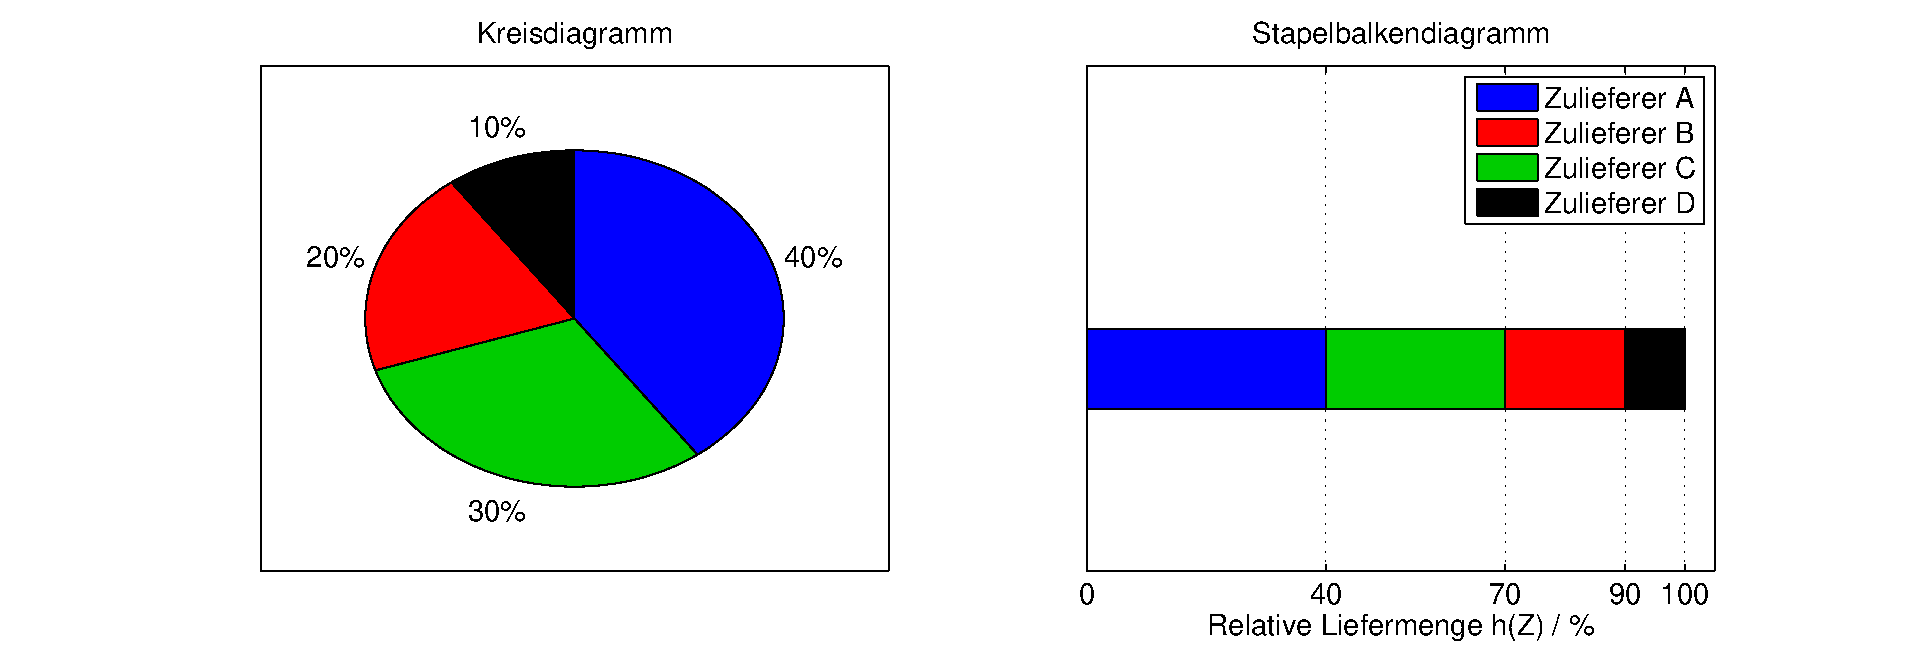
\includegraphics[width=1\textwidth]{Kapitel3/Bilder/image6}}
  \caption{Darstellung der relativen Liefermenge als Kreisdiagramm und als Stapelbalkendiagramm}
  \label{fig:Zuliefererbewertung1}
\end{figure}

\noindent Bei Darstellungen mithilfe von Kreis- oder Stapelbalkendiagrammen sollte darauf geachtet werden, dass der Kreis beziehungsweise der Balken nicht in zu viele Sektoren unterteilt wird, da sonst die \"{U}bersichtlichkeit des Diagrammes verloren geht. Es empfiehlt sich in diesem Fall, mehrere Sektoren zusammenzufassen. 

\noindent Ein Vergleich der einzelnen Zulieferer l\"{a}sst sich am besten mit einem einfachen Balkendiagramm erzielen. Dieses ist f\"{u}r die Werte aus Tabelle \ref{tab:threefour} in Bild \ref{fig:Zuliefererbewertung2} dargestellt.

\noindent 
\begin{figure}[H]
  \centerline{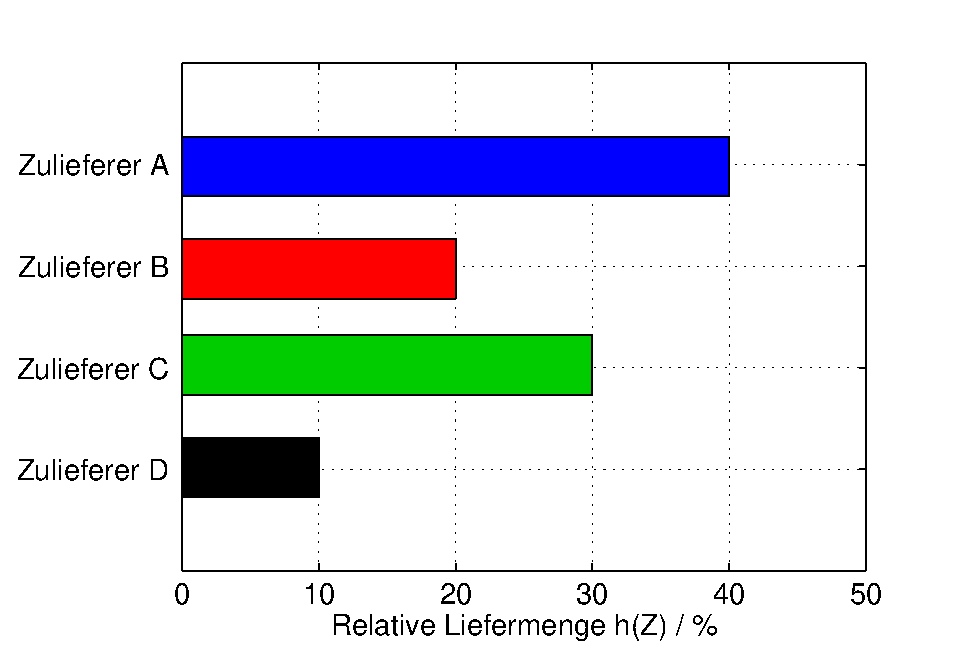
\includegraphics[width=0.5\textwidth]{Kapitel3/Bilder/image7}}
  \caption{Darstellung der relativen Liefermenge als Balkendiagramm}
  \label{fig:Zuliefererbewertung2}
\end{figure}

\noindent Bei dem Balkendiagramm in Bild \ref{fig:Zuliefererbewertung2} ist im Vergleich zu Bild \ref{fig:Zuliefererbewertung1} gut zu erkennen, dass Zulieferer A mit einem Lieferanteil von 40 \% das Vierfache von Zulieferer D liefert.

\clearpage

\subsubsection{Befehle zur Beschreibung von H\"{a}ufigkeiten in MATLAB}

\noindent Zur Berechnung und Darstellung von H\"{a}ufigkeitsverteilungen stehen in MATLAB diverse Funktionen zur Verf\"{u}gung. Die wichtigsten sind in Tabelle \ref{tab:threefive} zusammengefasst.

\begin{table}[H]
\setlength{\arrayrulewidth}{.1em}
\caption{Berechnung und Darstellung von H\"{a}ufigkeitsverteilungen in MATLAB}
\setlength{\fboxsep}{0pt}%
\colorbox{lightgray}{%
\arrayrulecolor{white}%
\begin{tabular}{| c | c |}
\hline
\parbox[c][0.3in][c]{3.3in}{\smallskip\centering\textbf{\fontfamily{phv}\selectfont{MATLAB Befehl}}} & 
\parbox[c][0.3in][c]{3.3in}{\smallskip\centering\textbf{\fontfamily{phv}\selectfont{Funktionsbeschreibung}}}\\ \hline

\parbox[c][0.3in][c]{3.3in}{\centering\fontfamily{phv}\selectfont{sort(x)}} & 
\parbox[c][0.3in][c]{3.3in}{\centering\fontfamily{phv}\selectfont{Sortiert die Werte des Vektors x nach der Gr\"{o}{\ss}e}}\\ \hline

\parbox[c][0.3in][c]{3.3in}{\centering\fontfamily{phv}\selectfont{cumsum(x)}} & 
\parbox[c][0.3in][c]{3.3in}{\centering\fontfamily{phv}\selectfont{Berechnet die kumulative Summe des Vektors x}}\\ \hline

\parbox[c][0.5in][c]{3.3in}{\centering\fontfamily{phv}\selectfont{hist(x)}} & 
\parbox[c][0.5in][c]{3.3in}{\centering\fontfamily{phv}\selectfont{Erzeugt ein Histogramm mit der absoluten H\"{a}ufigkeit von x}}\\ \hline

\parbox[c][0.3in][c]{3.3in}{\centering\fontfamily{phv}\selectfont{tabulate(x)}} & 
\parbox[c][0.3in][c]{3.3in}{\centering\fontfamily{phv}\selectfont{Erstellt eine H\"{a}ufigkeitstabelle aus x}}\\ \hline

\parbox[c][0.5in][c]{3.3in}{\centering\fontfamily{phv}\selectfont{bar(x)}} & 
\parbox[c][0.5in][c]{3.3in}{\centering\fontfamily{phv}\selectfont{Erzeugt ein Balkendiagramm ausx mit vertikaler Ausrichtung}}\\ \hline

\parbox[c][0.5in][c]{3.3in}{\centering\fontfamily{phv}\selectfont{barh(x)}} & 
\parbox[c][0.5in][c]{3.3in}{\centering\fontfamily{phv}\selectfont{Erzeugt ein Balkendiagramm ausX mit horizontaler Ausrichtung}}\\ \hline

\parbox[c][0.3in][c]{3.3in}{\centering\fontfamily{phv}\selectfont{pie(x)}} & 
\parbox[c][0.3in][c]{3.3in}{\centering\fontfamily{phv}\selectfont{Erzeugt ein Kreisdiagramm aus x}}\\ \hline

\end{tabular}%
}
\label{tab:threefive}
\end{table}

\subsubsection{Befehle zur Beschreibung von H\"{a}ufigkeiten in Python}

\noindent Zur Berechnung und Darstellung von H\"{a}ufigkeitsverteilungen stehen in Python diverse Funktionen zur Verf\"{u}gung. Die wichtigsten sind in Tabelle \ref{tab:threesix} zusammengefasst.

\begin{table}[H]
\setlength{\arrayrulewidth}{.1em}
\caption{Berechnung und Darstellung von H\"{a}ufigkeitsverteilungen in Python}
\setlength{\fboxsep}{0pt}%
\colorbox{lightgray}{%
\arrayrulecolor{white}%
\begin{tabular}{| c | c |}
\hline
\parbox[c][0.3in][c]{3.3in}{\smallskip\centering\textbf{\fontfamily{phv}\selectfont{Python Befehl}}} & 
\parbox[c][0.3in][c]{3.3in}{\smallskip\centering\textbf{\fontfamily{phv}\selectfont{Funktionsbeschreibung}}}\\ \hline

\parbox[c][0.3in][c]{3.3in}{\centering\fontfamily{phv}\selectfont{sorted}} & 
\parbox[c][0.3in][c]{3.3in}{\centering\fontfamily{phv}\selectfont{Sortiert die Werte des Vektors x nach der Gr\"{o}{\ss}e}}\\ \hline

\parbox[c][0.3in][c]{3.3in}{\centering\fontfamily{phv}\selectfont{numpy.cumsum}} & 
\parbox[c][0.3in][c]{3.3in}{\centering\fontfamily{phv}\selectfont{Berechnet die kumulative Summe des Vektors x}}\\ \hline

\parbox[c][0.5in][c]{3.3in}{\centering\fontfamily{phv}\selectfont{numpy.histogram}} & 
\parbox[c][0.5in][c]{3.3in}{\centering\fontfamily{phv}\selectfont{Erzeugt ein Histogramm mit der absoluten H\"{a}ufigkeit von x}}\\ \hline

\parbox[c][0.3in][c]{3.3in}{\centering\fontfamily{phv}\selectfont{count}} & 
\parbox[c][0.3in][c]{3.3in}{\centering\fontfamily{phv}\selectfont{Erstellt eine H\"{a}ufigkeitstabelle aus x}}\\ \hline

\parbox[c][0.5in][c]{3.3in}{\centering\fontfamily{phv}\selectfont{matplotlib.pyplot.bar}} & 
\parbox[c][0.5in][c]{3.3in}{\centering\fontfamily{phv}\selectfont{Erzeugt ein Balkendiagramm ausx mit vertikaler Ausrichtung}}\\ \hline

\parbox[c][0.5in][c]{3.3in}{\centering\fontfamily{phv}\selectfont{matplotlib.pyplot.barh}} & 
\parbox[c][0.5in][c]{3.3in}{\centering\fontfamily{phv}\selectfont{Erzeugt ein Balkendiagramm ausX mit horizontaler Ausrichtung}}\\ \hline

\parbox[c][0.3in][c]{3.3in}{\centering\fontfamily{phv}\selectfont{matplotlib.pyplot.pie}} & 
\parbox[c][0.3in][c]{3.3in}{\centering\fontfamily{phv}\selectfont{Erzeugt ein Kreisdiagramm aus x}}\\ \hline

\end{tabular}%
}
\label{tab:threesix}
\end{table}

\clearpage

\subsection{Kennwerte einer Stichprobe}

\noindent Jede Stichprobe wird mit ihrer H\"{a}ufigkeitsverteilung oder Summenh\"{a}ufigkeitsverteilung in allen Einzelheiten beschrieben. Gerade bei dem Vergleich gr\"{o}{\ss}erer Datenmengen sind diese H\"{a}ufigkeitsverteilungen aber unhandlich. Die Methoden der Statistik werden dazu verwendet, Stichproben \"{u}ber charakteristische Kenngr\"{o}{\ss}en oder Ma{\ss}zahlen abstrakt zu beschreiben. Dabei sind Kenngr\"{o}{\ss}en f\"{u}r die Lage, die Streuung und die Symmetrie einer Stichprobe zu unterscheiden. 

\subsubsection{Lagekennwerte einer Stichprobe}\label{threethreeone}

\noindent Lagekennwerte beschreiben die Lage des Zentrums einer Verteilung durch einen numerischen Wert.\bigskip

{\fontfamily{phv}\selectfont
\noindent\textbf{Arithmetischer Mittelwert einer Stichprobe}}\smallskip

\noindent Der arithmetische Mittelwert einer Stichprobe ist wohl die bekannteste Lagekenngr\"{o}{\ss}e. Er ist definiert als 

\begin{equation}\label{eq:threefifteen}
\bar{x}=\dfrac{x_{1} +{\rm \; ...\; }+x_{N} }{N} =\dfrac{1}{N} \cdot \sum _{n=1}^{N}x_{n}
\end{equation}

\noindent Liegen die Daten in Klassen mit ihren Klassenmitten $c_{n}$ vor, berechnet sich der arithmetische Mittelwert aus 

\begin{equation}\label{eq:threesixteen}
\bar{x}=\dfrac{c_{1} \cdot h_{A} (c_{1} )+{\rm \; ...\; }+c_{N} \cdot h_{A} (c_{N} )}{N} =\dfrac{1}{N} \cdot \sum _{n=1}^{N}(c_{n} \cdot h_{A} (c_{n})) =\sum _{n=1}^{N}(c_{n} \cdot h(c_{n}))
\end{equation}

Der arithmetische Mittelwert hat zwei wichtige Eigenschaften. Zum einen ist die Summe der Differenzen aller Werte von ihrem Mittelwert null. Diese Eigenschaft l\"{a}sst sich durch Zerlegen der Summe beweisen.

\begin{equation}\label{eq:threeseventeen}
\sum _{n=1}^{N}(x_{n} -\bar{x}) =\sum _{n=1}^{N}x_{n}  -\sum _{n=1}^{N}\bar{x} =\sum _{n=1}^{N}x_{n}  -N\cdot \bar{x}=N\cdot \bar{x}-N\cdot \bar{x}=0
\end{equation}

\noindent Zum anderen kann gezeigt werden, dass die Summe der Quadrate der Differenzen aller Werte von ihrem Mittelwert kleiner ist als die Summe der Quadrate der Differenzen aller Werte zu irgendeinem anderen Wert z. 

\begin{equation}\label{eq:threeeighteen}
\sum _{n=1}^{N}(x_{n} -\bar{x})^{2}  <\sum _{n=1}^{N}(x_{n} -z)^{2}
\end{equation}

\noindent Der arithmetische Mittelwert ist eine Kenngr\"{o}{\ss}e, die gerade bei kleinem Stichprobenumfang stark von einzelnen Ausrei{\ss}ern abh\"{a}ngig sein kann.

\clearpage

\noindent
\colorbox{lightgray}{%
\arrayrulecolor{white}%
\renewcommand\arraystretch{0.6}%
\begin{tabular}{ wl{16.5cm} }
{\fontfamily{phv}\selectfont
\noindent{Beispiel: Kapazit\"{a}tsmessung}}
\end{tabular}%
}\bigskip

\noindent Als Beispiel sind in Tabelle \ref{tab:threeseven} zwei Messreihen dargestellt, in denen jeweils N = 10 Kondensatoren mit einem nominalen Kapazit\"{a}tswert von C = 100 nF vermessen wurden. In der zweiten Messreihe wurde ein Messwert durch einen Ausrei{\ss}er ersetzt.

\begin{table}[H]
\setlength{\arrayrulewidth}{.1em}
\caption{Beispiel f\"{u}r eine Urliste: Messwerte von 100 Widerst\"{a}nden mit einem Sollwert von $R = 1 k \Omega $}
\setlength{\fboxsep}{0pt}%
\colorbox{lightgray}{%
\arrayrulecolor{white}%
\begin{tabular}{wc{0cm}  wl{0.9cm} | wc{1.3cm} | wc{1.3cm} | wc{1.3cm} | wc{1.3cm} | wc{1.3cm} | wc{1.3cm} | wc{1.3cm} | wc{1.3cm} | wc{1.3cm} }
\hline\xrowht{15pt}

& \multicolumn{10}{c}{\fontfamily{phv}\selectfont\textbf{Messreihe 1: Kapazit\"{a}tswerte C / nF}} \\ \hline \xrowht{15pt}

& 101 & 102 & 99 & 98 & 100 & 97 & 99 & 100 & 101 & 103\\ \hline\xrowht{15pt}

& \multicolumn{10}{c}{\fontfamily{phv}\selectfont\textbf{Messreihe 2: Kapazit\"{a}tswerte C / nF}} \\ \hline \xrowht{15pt}

& 101 & 153 & 99 & 98 & 100 & 97 & 99 & 100 & 101 & 103 \\ \hline

\end{tabular}%
}
\label{tab:threeseven}
\end{table}

\noindent Der arithmetische Mittelwert f\"{u}r Messreihe 1 ergibt sich aus 

\begin{equation}\label{eq:threenineteen}
\overline{C}_{1} =\dfrac{1}{N} \cdot \sum _{n=1}^{N}C_{n,1}  =\dfrac{101+102+...+103}{10} nF= 100 nF
\end{equation}

\noindent Wegen des Messfehlers in der zweiten Messreihe weicht der arithmetische Mittelwert stark von dem nominellen Wert ab. F\"{u}r Messreihe 2 ergibt sich der Mittelwert zu

\begin{equation}\label{eq:threetwenty}
\overline{C}_{2} =\dfrac{1}{N} \cdot \sum _{n=1}^{N}C_{n,2}  =\dfrac{101+153+...+103}{10} nF= 105.1 nF
\end{equation}

\noindent Das Beispiel best\"{a}tigt die Empfindlichkeit des arithmetischen Mittelwertes gegen\"{u}ber Ausrei{\ss}ern. Mit fallendem Stichprobenumfang steigt der Einfluss der Fehlmessung weiter an. \bigskip

{\fontfamily{phv}\selectfont
\noindent\textbf{Median einer Stichprobe}}\smallskip

\noindent Ein Lagema{\ss}, das weniger empfindlich auf Ausrei{\ss}er reagiert als der arithmetische Mittelwert, ist der Median. Der Median $x_{MED}$ ist der Wert, bei dem die H\"{a}lfte der Stichprobenwerte x gr\"{o}{\ss}er und die H\"{a}lfte der Stichprobenwerte x kleiner ist. 

\begin{equation}\label{eq:threetwentyone}
H(x_{MED})=0.5
\end{equation}

\noindent Bei ungeradem Stichprobenumfang n ist der Median $x_{MED}$ der mittlere Wert der nach Gr\"{o}{\ss}e geordneten Stichprobe. Bei geradem Stichprobenumfang ergibt sich der Median aus dem Mittelwert der beiden Stichprobenwerte, die in der Mitte der geordneten Stichprobe liegen.

\clearpage

\noindent
\colorbox{lightgray}{%
\arrayrulecolor{white}%
\renewcommand\arraystretch{0.6}%
\begin{tabular}{ wl{16.5cm} }
{\fontfamily{phv}\selectfont
\noindent{Beispiel: Kapazit\"{a}tsmessung}}
\end{tabular}%
}\bigskip

\noindent Zur Bestimmung des Medians f\"{u}r die Messreihen aus Tabelle \ref{tab:threeseven} m\"{u}ssen die Daten zun\"{a}chst sortiert werden.

\begin{table}[H]
\setlength{\arrayrulewidth}{.1em}
\caption{Beispiel f\"{u}r eine Urliste: Messwerte von 100 Widerst\"{a}nden mit einem Sollwert von $R = 1 k \Omega $}
\setlength{\fboxsep}{0pt}%
\colorbox{lightgray}{%
\arrayrulecolor{white}%
\begin{tabular}{wc{0cm}  wl{0.9cm} | wc{1.3cm} | wc{1.3cm} | wc{1.3cm} | wc{1.3cm} | wc{1.3cm} | wc{1.3cm} | wc{1.3cm} | wc{1.3cm} | wc{1.3cm} }
\hline\xrowht{15pt}

& \multicolumn{10}{c}{\fontfamily{phv}\selectfont\textbf{Messreihe 1: Kapazit\"{a}tswerte C / nF}} \\ \hline \xrowht{15pt}

& 97 & 98 & 99 & 99 & 100 & 100 & 101 & 101 & 102 & 103\\ \hline\xrowht{15pt}

& \multicolumn{10}{c}{\fontfamily{phv}\selectfont\textbf{Messreihe 2: Kapazit\"{a}tswerte C / nF}} \\ \hline \xrowht{15pt}

& 97 & 98 & 99 & 99 & 100 & 100 & 101 & 101 & 103 & 153 \\ \hline

\end{tabular}%
}
\label{tab:threeeight}
\end{table}

\noindent Aus den Messreihen 1 und 2 ergeben sich die beiden Mediane aus den arithmetischen Mittelwerten des f\"{u}nften und sechsten Elementes zu 

\begin{equation}\label{eq:threetwentytwo}
C_{MED,1} =\dfrac{C_{5,1} +C_{6,1} }{2} = 100 nF
\end{equation}

\noindent beziehungsweise

\begin{equation}\label{eq:threetwentythree}
C_{MED,2} =\dfrac{C_{5,2} +C_{6,2} }{2} = 100 nF
\end{equation}

\noindent Das Beispiel zeigt, dass der Median deutlich unempfindlicher auf Messausrei{\ss}er reagiert als der arithmetische Mittelwert, in diesem Beispiel bleibt er sogar konstant. F\"{u}r den Median ist zum Beispiel der Absolutwert des gr\"{o}{\ss}ten und des kleinsten Stichprobenwertes v\"{o}llig gleichg\"{u}ltig. Der Median wird deshalb als resistenter oder robuster Lagekennwert bezeichnet.\newline

\noindent Liegen die Daten in gruppierter Form mit konstanter Klassenbreite d vor, kann die relative Lage des Medians in der Klasse ber\"{u}cksichtigt werden. Dazu wird zwischen den benachbarten Klassenmitten $c_{n}$ ein linearer Zusammenhang zwischen der Summenh\"{a}ufigkeit H(x) und dem Merkmal x angenommen. Bild \ref{fig:MedianKlassen}
stellt diese Annahme grafisch dar.

\noindent 
\begin{figure}[H]
  \centerline{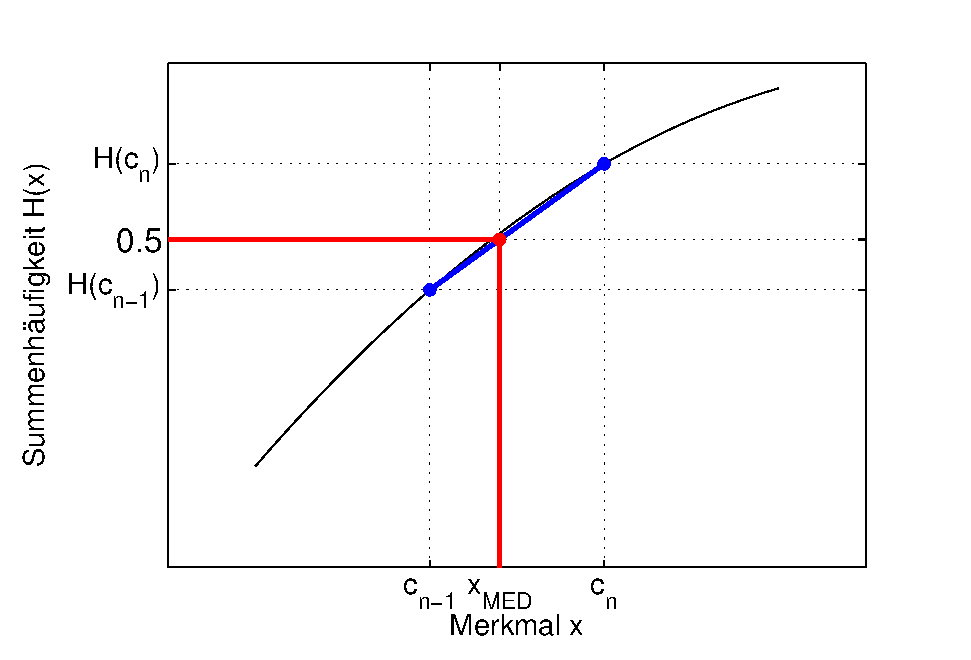
\includegraphics[width=0.5\textwidth]{Kapitel3/Bilder/image8}}
  \caption{Lineare Interpolation zwischen Summenh\"{a}ufigkeit H(x) und Merkmal x}
  \label{fig:MedianKlassen}
\end{figure}

\noindent Die Steigung der Geraden zwischen den bekannten Werten f\"{u}r die Klassenmitten ergibt sich aus 

\begin{equation}\label{eq:threetwentyfour}
m=\dfrac{H(c_{n})-H(c_{n-1})}{c_{n} -c_{n-1} } =\dfrac{h(c_{n})}{d}
\end{equation}

\noindent Daraus folgt f\"{u}r die Summenh\"{a}ufigkeit des Medians die Geradengleichung

\begin{equation}\label{eq:threetwentyfive}
H(x_{MED})=0.5=H(c_{n-1})+m\cdot (x_{MED} -c_{n-1} )=H(c_{n-1})+\dfrac{h(c_{n} )}{d} \cdot (x_{MED} -c_{n-1})
\end{equation}

\noindent Sie kann nach dem Median aufgel\"{o}st werden. Es ergibt sich 

\begin{equation}\label{eq:threetwentysix}
x_{MED} =c_{n-1} +\dfrac{d\cdot(0.5-H(c_{n-1}))}{h(c_{n})}
\end{equation}

\noindent
\colorbox{lightgray}{%
\arrayrulecolor{white}%
\renewcommand\arraystretch{0.6}%
\begin{tabular}{ wl{16.5cm} }
{\fontfamily{phv}\selectfont
\noindent{Beispiel: Widerstandsmessung}}
\end{tabular}%
}\bigskip

\noindent F\"{u}r das Beispiel aus Tabelle 3.3 ergibt sich damit als Median 

\begin{equation}\label{eq:threetwentyseven}
R_{MED} =985\Omega +\dfrac{1\Omega \cdot (0.5-0.23)}{0.32} = 985.84 \Omega
\end{equation}

\noindent Der Wert erreicht eine Aufl\"{o}sung, die unterhalb der Klassenbreite d liegt. Sowohl das arithmetische Mittel als auch der Median m\"{u}ssen bei diskreten Datentypen nicht mit einer m\"{o}glichen Auspr\"{a}gung $x_{n}$ \"{u}bereinstimmen. Liegt der Median genau auf der Grenze zweier Klassen, kann diese Rechnung nicht durchgef\"{u}hrt werden. In diesem Fall entspricht der Median der Grenze der beiden Klassen.\bigskip

{\fontfamily{phv}\selectfont
\noindent\textbf{Weitere Lagekennwerte von Stichproben}}\smallskip

\noindent Neben dem arithmetischen Mittelwert und dem Median sind zwei weitere Kennwerte gebr\"{a}uchlich. Bei Wachstumsprozessen wird das geometrische Mittel $x_{G}$ verwendet, das sich bei einem Stichprobenumfang N aus der N-ten Wurzel des Produktes der einzelnen Stichprobenwerte berechnet.

\begin{equation}\label{eq:threetwentyeight}
x_{G} =\sqrt[{N}]{x_{1} \cdot {\rm \; ...\; }\cdot x_{N} } =\sqrt[{N}]{\prod _{i=1}^{N}x_{n}}
\end{equation}

\noindent Der Modus ist der am h\"{a}ufigsten vorkommende Wert einer Stichprobe, also der Wert mit der gr\"{o}{\ss}ten absoluten oder relativen H\"{a}ufigkeit. Auf beide Kennwerte wird hier nicht weiter eingegangen.

\clearpage

{\fontfamily{phv}\selectfont
\noindent\textbf{Zusammenfassung der Lagekennwerte von Stichproben}}\smallskip

\noindent Zur besseren \"{U}bersicht fasst Tabelle \ref{tab:threenine} die Lagekennwerte einer Stichprobe zusammen.

\begin{table}[H]
\setlength{\arrayrulewidth}{.1em}
\caption{Lagekennwerte einer Stichprobe}
\setlength{\fboxsep}{0pt}%
\colorbox{lightgray}{%
\arrayrulecolor{white}%
\begin{tabular}{| wc{5.5cm} | wc{5.5cm} | wc{5.5cm} }
\xrowht{15pt}

{\fontfamily{phv}\selectfont\textbf{Lagekennwert}} & 
{\fontfamily{phv}\selectfont\textbf{Definition}} &
{\fontfamily{phv}\selectfont\textbf{Bemerkungen}}\\ \hline \xrowht{35pt}

{\fontfamily{phv}\selectfont{Mittelwert}} &
$\bar{x}=\dfrac{x_{1} +{\rm \; ...\; }+x_{N} }{N} =\dfrac{1}{N} \cdot \sum _{n=1}^{N}x_{n}$ &
\multirow{4}{5cm}{\centering\fontfamily{phv}\selectfont{Empfindlich gegen\"{u}ber Ausrei{\ss}ern}}\\ 
\cline{1-2}\xrowht{35pt}
{\fontfamily{phv}\selectfont{Mittelwert von Daten in Klassen}} & 
$\bar{x}=\sum _{n=1}^{N}\left(x_{n} \cdot h(c_{n} )\right)$ & \\ \hline \xrowht{20pt}

{\fontfamily{phv}\selectfont{Median}} &
$H\left(x_{MED} \right)=0.5$ &
\multirow{5}{5cm}{\centering\fontfamily{phv}\selectfont{Weniger empfindlich gegen\"{u}ber Ausrei{\ss}ern als der Mittelwert}}\\ 
\cline{1-2}\xrowht{45pt}
{\fontfamily{phv}\selectfont{Median von Daten in Klassen}} & 
$x_{MED} =c_{n-1} +\dfrac{d\cdot \left(0.5-H\left(c_{n-1} \right)\right)}{h\left(c_{n} \right)} $ & \\ \hline \xrowht{20pt}

{\fontfamily{phv}\selectfont{Geometrisches Mittel}} &
$x_{G} =\sqrt[{N}]{x_{1} \cdot {\rm \; ...\; }\cdot x_{N} } $ & \\ \hline \xrowht{20pt}

{\fontfamily{phv}\selectfont{Modus}} &
{\fontfamily{phv}\selectfont{häufigster Wert einer Stichprobe}} & \\ \hline 

\end{tabular}%
}\bigskip
\label{tab:threenine}
\end{table}

\noindent Da zur Berechnung der Lagekennwerte meist entsprechende Software verwendet wird, ent-fällt in vielen Fällen eine Einteilung der Daten in Klassen. MATLAB bietet einige Funktionen, mit denen die Lagekennwerte von Stichproben bestimmt werden können. Sie sind in Tabelle \ref{tab:threeten} aufgelistet.

\begin{table}[H]
\setlength{\arrayrulewidth}{.1em}
\caption{Berechnung der Lagekennwerte von Stichproben in MATLAB}
\setlength{\fboxsep}{0pt}%
\colorbox{lightgray}{%
\arrayrulecolor{white}%
\begin{tabular}{| c | c |}
\hline
\parbox[c][0.3in][c]{3.3in}{\smallskip\centering\textbf{\fontfamily{phv}\selectfont{Lagekennwert}}} & 
\parbox[c][0.3in][c]{3.3in}{\smallskip\centering\textbf{\fontfamily{phv}\selectfont{MATLAB-Befehl}}}\\ \hline

\parbox[c][0.3in][c]{3.3in}{\centering\fontfamily{phv}\selectfont{Mittelwert}} & 
\parbox[c][0.3in][c]{3.3in}{\centering\fontfamily{phv}\selectfont{mean(X)}}\\ \hline

\parbox[c][0.3in][c]{3.3in}{\centering\fontfamily{phv}\selectfont{Median}} & 
\parbox[c][0.3in][c]{3.3in}{\centering\fontfamily{phv}\selectfont{median(x)}}\\ \hline

\parbox[c][0.3in][c]{3.3in}{\centering\fontfamily{phv}\selectfont{Geometrisches Mittel }} & 
\parbox[c][0.3in][c]{3.3in}{\centering\fontfamily{phv}\selectfont{geomean(X)}}\\ \hline

\parbox[c][0.3in][c]{3.3in}{\centering\fontfamily{phv}\selectfont{Modus}} & 
\parbox[c][0.3in][c]{3.3in}{\centering\fontfamily{phv}\selectfont{mode(X)}}\\ \hline

\end{tabular}%
}
\label{tab:threeten}
\end{table}

\noindent Vergleichbare Befehle existieren in Python, sie sind in Tabelle \ref{tab:threeeleven} zusammengestellt.

\begin{table}[H]
\setlength{\arrayrulewidth}{.1em}
\caption{Berechnung der Lagekennwerte von Stichproben in Python}
\setlength{\fboxsep}{0pt}%
\colorbox{lightgray}{%
\arrayrulecolor{white}%
\begin{tabular}{| c | c |}
\hline
\parbox[c][0.3in][c]{3.3in}{\smallskip\centering\textbf{\fontfamily{phv}\selectfont{Lagekennwert}}} & 
\parbox[c][0.3in][c]{3.3in}{\smallskip\centering\textbf{\fontfamily{phv}\selectfont{MATLAB-Befehl}}}\\ \hline

\parbox[c][0.3in][c]{3.3in}{\centering\fontfamily{phv}\selectfont{Mittelwert}} & 
\parbox[c][0.3in][c]{3.3in}{\centering\fontfamily{phv}\selectfont{numpy.median}}\\ \hline

\parbox[c][0.3in][c]{3.3in}{\centering\fontfamily{phv}\selectfont{Median}} & 
\parbox[c][0.3in][c]{3.3in}{\centering\fontfamily{phv}\selectfont{numpy.mean}}\\ \hline

\parbox[c][0.3in][c]{3.3in}{\centering\fontfamily{phv}\selectfont{Geometrisches Mittel }} & 
\parbox[c][0.3in][c]{3.3in}{\centering\fontfamily{phv}\selectfont{scipy.stats.mstats.gmean}}\\ \hline

\parbox[c][0.3in][c]{3.3in}{\centering\fontfamily{phv}\selectfont{Modus}} & 
\parbox[c][0.3in][c]{3.3in}{\centering\fontfamily{phv}\selectfont{scipy.stats.mode}}\\ \hline

\end{tabular}%
}
\label{tab:threeeleven}
\end{table}

\subsubsection{Streuungskennwerte einer Stichprobe}\label{threethreetwo}

\noindent Der Mittelwert und der Median sind Kennwerte für die Lage einer Stichprobe. Für eine zu-sammenfassende Beschreibung ist es notwendig, zusätzlich die Streuung der Stichprobe zu charakterisieren. Dazu können Spannweite, Varianz und Quantile der Verteilung verwendet werden.\bigskip

{\fontfamily{phv}\selectfont
\noindent\textbf{Spannweite}}\smallskip

\noindent Die Spannweite oder Streu- beziehungsweise Variationsbreite einer Stichprobe ergibt sich aus der Differenz von gr\"{o}{\ss}tem und kleinstem Stichprobenwert. 

\begin{equation}\label{eq:threetwentynine}
\Delta x=x_{MAX} -x_{MIN}
\end{equation}

\noindent
\colorbox{lightgray}{%
\arrayrulecolor{white}%
\renewcommand\arraystretch{0.6}%
\begin{tabular}{ wl{16.5cm} }
{\fontfamily{phv}\selectfont
\noindent{Beispiel: Kapazit\"{a}tsmessung}}
\end{tabular}%
}\bigskip

\noindent F\"{u}r die Messreihen 1 und 2 aus Tabelle \ref{tab:threeseven} ergeben sich die beiden Spannweiten zu 

\begin{equation}\label{eq:threethirty}
\Delta C_{1} = 103 nF-97 nF=6 nF
\end{equation}

\noindent beziehungsweise 

\begin{equation}\label{eq:threethirtyone}
\Delta C_{2} = 153 nF - 97 nF = 56 nF
\end{equation}

\noindent Die Spannweite reagiert offensichtlich extrem auf Ausrei{\ss}er und besitzt damit bez\"{u}glich der Streuung aller Stichprobenwerte nur eine geringe Aussagekraft.\bigskip

{\fontfamily{phv}\selectfont
\noindent\textbf{Varianz und Standardabweichung}}

\noindent Die Varianz betrachtet die Streuung aller Stichprobenwerte um den Mittelwert. Die Summe der einzelnen Abweichungen heben sich auf.

\begin{equation}\label{eq:threethirtytwo}
\sum _{n=1}^{N}(x_{n} -\bar{x})= \sum _{n=1}^{N}x_{n} -N\cdot \bar{x}= 0
\end{equation}

\noindent Der Mittelwert kann deshalb nicht zur Bewertung der Streuung herangezogen werden. Eine bessere M\"{o}glichkeit zur Bestimmung der Streuung einer Stichprobe ergibt sich aus der Summe der quadrierten Abweichungen. Durch das Quadrieren werden alle Elemente der Summe positiv und k\"{o}nnen sich nicht mehr gegenseitig kompensieren. Es ergibt sich die Varianz $s^{2}$, die definiert ist als

\begin{equation}\label{eq:threethirtythree}
s^{2} =\dfrac{1}{N-1} \cdot \sum _{n=1}^{N}\left(x_{n} -\bar{x}\right)^{2}
\end{equation}

\noindent F\"{u}r eine manuelle Berechnung kann Gleichung \eqref{eq:threethirtythree} mit der binomischen Formel umgeformt werden zu

\begin{equation}\label{eq:threethirtyfour}
\begin{split}
s^{2}  & = \dfrac{1}{N-1} \cdot \sum _{n=1}^{N}(x_{n} -\bar{x})^{2}  =\dfrac{1}{N-1} \cdot \sum _{n=1}^{N}(x_{n}^{2} -2\cdot x_{n} \cdot \bar{x}+\bar{x}^{2} ) \\ 
& = \dfrac{1}{N-1} \cdot \left(\sum _{n=1}^{N} x^{2}_{n} - 2\cdot N \cdot \bar{x}^{2} + N\cdot \bar{x}^{2} \right) =  \dfrac{1}{N-1} \cdot  \left(\sum _{n=1}^{N} x^{2}_{n} -   N\cdot \bar{x}^{2} \right)
\end{split}
\end{equation}

\noindent Im Gegensatz zu dem Mittelwert wird bei der Varianz nicht durch die Anzahl N der Stichprobenwerte, sondern durch den Wert (N -- 1) geteilt. Mathematisch ergibt sich die Division durch den Wert (N -- 1) dadurch, dass bei der Bildung der Varianz die Differenzen zum Mittelwert ausgewertet werden. Der Mittelwert wird bereits mit diesen Daten berechnet, sodass ein Summand in Gleichung \eqref{eq:threethirtytwo} sich aus den \"{u}brigen (N -- 1) Werten ergibt. Es sind also nur (N -- 1) Summanden unabh\"{a}ngig oder frei. Es geht ein sogenannter Freiheitsgrad verloren, sodass die Division durch den Wert (N -- 1) gerechtfertigt ist. \bigskip

\noindent
\colorbox{lightgray}{%
\arrayrulecolor{white}%
\renewcommand\arraystretch{0.6}%
\begin{tabular}{ wl{16.5cm} }
{\fontfamily{phv}\selectfont
\noindent{Beispiel: Kapazit\"{a}tsmessung}}
\end{tabular}%
}\bigskip

\noindent F\"{u}r die Messreihen 1 und 2 aus Tabelle \ref{tab:threeseven} ergeben sich die beiden Varianzen zu 

\begin{equation}\label{eq:threethirtyfive}
s_{C1}^{2} = 3.33 n{F}^{2}
\end{equation}

\noindent beziehungsweise 

\begin{equation}\label{eq:threethirtysix}
s_{C2}^{2} = 286.1 n{F}^{2}
\end{equation}

\noindent Die Varianz ist ein Ma{\ss} f\"{u}r die Streuung, der physikalische Gehalt der Gr\"{o}{\ss}e ist aber unanschaulich. Aus diesem Grund wird f\"{u}r die Kennzeichnung einer Streuung oft die Standardabweichung verwendet. Die Standardabweichung s ergibt sich aus der positiven Quadratwurzel der Varianz $s^{2}$ und berechnet sich aus 

\begin{equation}\label{eq:threethirtyseven}
s=\sqrt{\dfrac{1}{N-1} \cdot \sum _{n=1}^{N}(x_{n} -\bar{x})^{2}}
\end{equation}

\noindent Die Standardabweichung hat dieselbe physikalische Dimension wie die Stichprobenwerte x und eignet sich damit gut f\"{u}r eine anschauliche Interpretation.\bigskip

\noindent
\colorbox{lightgray}{%
\arrayrulecolor{white}%
\renewcommand\arraystretch{0.6}%
\begin{tabular}{ wl{16.5cm} }
{\fontfamily{phv}\selectfont
\noindent{Beispiel: Kapazit\"{a}tsmessung}}
\end{tabular}%
}\bigskip

\noindent F\"{u}r die Messreihen 1 und 2 aus Tabelle \ref{tab:threeseven} ergeben sich die beiden Varianzen zu 

\begin{equation}\label{eq:threethirtyeight}
s_{C1}^{2} = 1.825 nF
\end{equation}

\noindent beziehungsweise 

\begin{equation}\label{eq:threethirtynine}
s_{C2}^{2} = 16.915 nF
\end{equation} 

\noindent Liegt die Stichprobe in Klassen vor, ergibt sich die Varianz aus 

\begin{equation}\label{eq:threefourty}
s^{2} =\dfrac{1}{N-1} \cdot \sum _{n=1}^{N}\left(h_{A} (c_{n})\cdot (c_{n} -\bar{x})^{2} \right)
\end{equation} 

\noindent und die Standardabweichung berechnet sich entsprechend zu

\begin{equation}\label{eq:threefourtyone}
s=\sqrt{\dfrac{1}{N-1} \cdot \sum _{n=1}^{N}\left(h_{A} (c_{n})\cdot (c_{n} -\bar{x})^{2} \right)}
\end{equation} 

{\fontfamily{phv}\selectfont
\noindent\textbf{Quantilabst\"{a}nde einer Stichprobe}}

\noindent Auch wenn die Empfindlichkeit der Varianz gegen\"{u}ber Ausrei{\ss}ern kleiner ist als die der Spannweite einer Stichprobe, reagiert die Standardabweichung auf Ausrei{\ss}er \"{a}hnlich stark wie der arithmetische Mittelwert. Aus diesem Grund werden Streuungskenngr\"{o}{\ss}en definiert, die sich an der Definition des Medians orientieren und als Quantile bezeichnet werden. Das P-Quantil $x_{P}$ einer Verteilung trennt die Daten so in zwei Teile, dass ein Anteil P unterhalb des Quantils liegt und ein Anteil (1 -- P) \"{u}ber dem Quantil liegt. 

\begin{equation}\label{eq:threefourtytwo}
H(x_{P})=P
\end{equation} 

\noindent Der Median entspricht dem 50\%-Quantil. Werden die Quantile die Stichprobe in vier Intervalle teilen, werden Sie als Quartile bezeichnet. Die Quartile eine Stichprobe lassen sich \"{a}hnlich wie der Median einer Stichprobe bestimmen. Auch die Rechenregeln f\"{u}r in Klassen eingeteilte Daten mit konstanter Klassenbreite d gelten sinngem\"{a}{\ss}, sodass die Quartile bestimmt werden durch

\begin{equation}\label{eq:threefourtythree}
x_{0.25} =c_{n-1} +\dfrac{d\cdot (0.25-H(c_{n-1}))}{h(c_{n})}
\end{equation} 

\begin{equation}\label{eq:threefourtyfour}
x_{0.75} =c_{n-1} +\dfrac{d\cdot (0.75-H(c_{n-1}))}{h(c_{n})}
\end{equation} 

\noindent Dar\"{u}ber hinaus ist eine grafische Bestimmung der Quartile aus der Summenh\"{a}ufigkeit m\"{o}glich. 

\noindent Der Abstand zwischen dem 75\%- und dem 25\%-Quartil wird als Interquartilabstand (inter quartile range) IQR bezeichnet. 

\begin{equation}\label{eq:threefourtyfive}
IQR=x_{0.75} -x_{0.25}
\end{equation} 

\noindent Der Interquartilabstand ist unempfindlich gegen Ausrei{\ss}er, weil er von der absoluten Lage der Stichprobenwerte, die am Rand der Verteilung liegen, unabh\"{a}ngig ist.

\clearpage

\noindent
\colorbox{lightgray}{%
\arrayrulecolor{white}%
\renewcommand\arraystretch{0.6}%
\begin{tabular}{ wl{16.5cm} }
{\fontfamily{phv}\selectfont
\noindent{Beispiel: Widerstandsmessung}}
\end{tabular}%
}\bigskip

\noindent Die Berechnung wird am Beispiel der Widerstandsmessung veranschaulicht. Bild \ref{fig:SummenhQuantileStichprobeWiderstand} zeigt die Summenh\"{a}ufigkeit der Stichprobe aus Tabelle 3.1 sowie die 25\%-, 50\%- und 75\%-Quantile der Stichprobe. 

\noindent 
\begin{figure}[H]
  \centerline{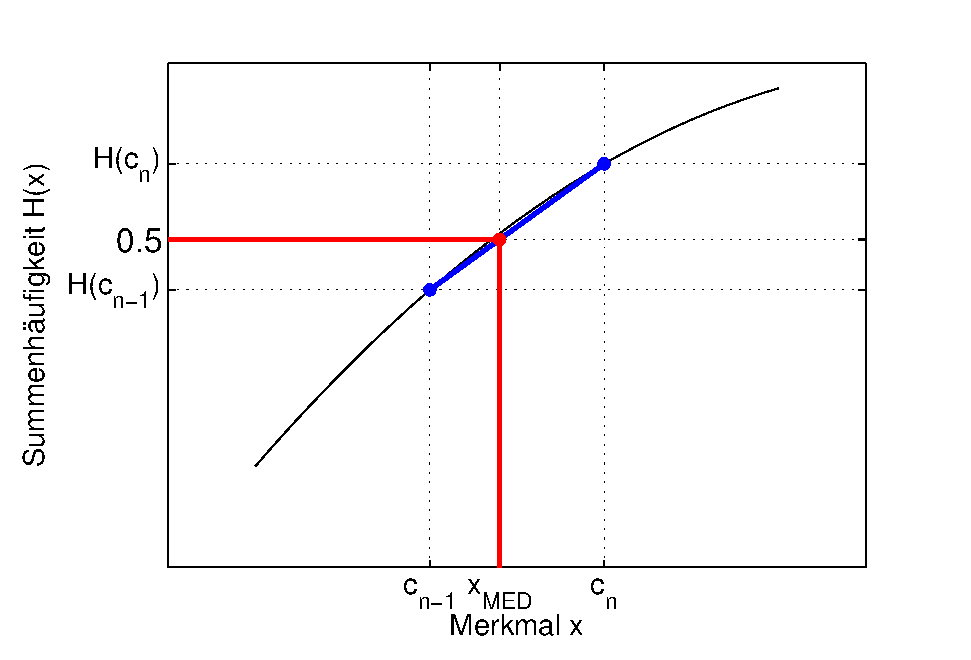
\includegraphics[width=0.5\textwidth]{Kapitel3/Bilder/image8}}
  \caption{Darstellung der Summenh\"{a}ufigkeit f\"{u}r die Stichprobe in Tabelle \ref{tab:threethree} mit Quartilen }
  \label{fig:SummenhQuantileStichprobeWiderstand}
\end{figure}

\noindent F\"{u}r die Daten in Tabelle \ref{tab:threethree} ergeben sich das 25\%- und 75\%-Quartil zu 

\begin{equation}\label{eq:threefourtysix}
R_{0.25} =985 \Omega +\dfrac{1 \Omega \cdot (0.25-0.23)}{0.32} = 985.06 \Omega
\end{equation} 

\begin{equation}\label{eq:threefourtyseven}
R_{0.75} =987 \Omega +\dfrac{1 \Omega \cdot (0.75-0.72)}{0.15} = 987.20 \Omega
\end{equation} 

\noindent Damit errechnet sich der Inter-Quartil-Range zu

\begin{equation}\label{eq:threefourtyeight}
IQR=R_{0.75} -R_{0.25} = 987.20 \Omega - 985.06 \Omega =2.14 \Omega 
\end{equation} 

\clearpage

{\fontfamily{phv}\selectfont
\noindent\textbf{Zusammenfassung der Streuungskennwerte von Stichproben}}

\noindent Zur besseren \"{U}bersicht fasst Tabelle \ref{tab:threetwelve} die Streuungskennwerte einer Stichprobe zusammen.

\begin{table}[H]
\setlength{\arrayrulewidth}{.1em}
\caption{Berechnung der Lagekennwerte von Stichproben in Python}
\setlength{\fboxsep}{0pt}%
\colorbox{lightgray}{%
\arrayrulecolor{white}%
\begin{tabular}{| wc{5.5cm} | wc{5.5cm} | wc{13em} }
\xrowht{15pt}

{\fontfamily{phv}\selectfont\textbf{Streuungskennwert}} & 
{\fontfamily{phv}\selectfont\textbf{Definition}} &
{\fontfamily{phv}\selectfont\textbf{Bemerkungen}}\\ \hline \xrowht{20pt}

\multirow{3}{*}{\fontfamily{phv}\selectfont{Spannweite}} &
\multirow{3}{*}{$\Delta x=x_{MAX} -x_{MIN} $} &
{\fontfamily{phv}\selectfont{Extrem empfindlich}} \\ \xrowht{20pt}
& & {\fontfamily{phv}\selectfont{gegenüber Ausreißern}}\\ \hline \xrowht{35pt}

{\fontfamily{phv}\selectfont{Varianz}} &
$s^{2} =\dfrac{1}{N-1} \cdot \sum _{n=1}^{N}(x_{n} -\bar{x})^{2}$ &
\multirow{5}{5cm}{\centering\fontfamily{phv}\selectfont{Empfindlich gegen\"{u}ber Ausrei{\ss}ern}}\\ \cline{1-2}\xrowht{15.5pt}
\fontfamily{phv}\selectfont{Varianz in Klassen} & \multirow{3}{*}{$s^{2} =\dfrac{1}{N-1} \cdot \sum _{n=1}^{N}\left(h_{A} (c_{n})\cdot (c_{n} -\bar{x}\right)^{2})$}&\\ \xrowht{15.5pt}
\fontfamily{phv}\selectfont{eingeteilter Daten} & & \\ \hline \xrowht{45pt}

{\fontfamily{phv}\selectfont{Standardabweichung}} &
$s=\sqrt{\dfrac{1}{N-1} \cdot \sum _{n=1}^{N}(x_{n} -\bar{x})^{2}}$ &
\multirow{5}{5cm}{\centering\fontfamily{phv}\selectfont{ Vergleichbar zur Varianz, aber in Einheiten der Zielgr\"{o}{\ss}e x}}\\ 
\cline{1-2}\xrowht{22.5pt}
\fontfamily{phv}\selectfont{Standardabweichungin Klassen} & \multirow{3}{*}{$s=\sqrt{\dfrac{1}{N-1} \cdot \sum _{n=1}^{N}\left(h_{A} \left(c_{n} \right)\cdot \left(c_{n} -\bar{x}\right)^{2} \right)}$}&\\ \xrowht{22.5pt}
\fontfamily{phv}\selectfont{eingeteilter Daten} & & \\ \hline\xrowht{20pt}

{\fontfamily{phv}\selectfont{P-Quantil}} &
$H\left(x_{P} \right)=P$ & \\ \hline \xrowht{15pt}

\fontfamily{phv}\selectfont{P-Quantilin Klassen} & \multirow{3}{*}{$x_{P} =c_{n-1} +\dfrac{d\cdot \left(P-H\left(c_{n-1} \right)\right)}{h\left(c_{n} \right)} $}&\\ \xrowht{15pt}
\fontfamily{phv}\selectfont{eingeteilter Daten} & & \\ \hline \xrowht{20pt}

{\fontfamily{phv}\selectfont{Interquartilabstand}} &
$IQR=x_{0.75} -x_{0.25} $ & 
{\fontfamily{phv}\selectfont{Robuster Streuungskennwert}} \\ \hline 

\end{tabular}%
}\bigskip
\label{tab:threetwelve}
\end{table}

\noindent Gerade bei gr\"{o}{\ss}eren Stichprobenumf\"{a}ngen ist es aufwendig, die Streuungskennwerte manuell zu berechnen. Daher wird zur Auswertung meist entsprechende Software herangezogen. Die Befehle zur Berechnung der Streuungskenngr\"{o}{\ss}en mit MATLAB sind in Tabelle \ref{tab:threethirteen} zusammengefasst.

\begin{table}[H]
\setlength{\arrayrulewidth}{.1em}
\caption{Berechnung der Streuungskennwerte von Stichproben in MATLAB}
\setlength{\fboxsep}{0pt}%
\colorbox{lightgray}{%
\arrayrulecolor{white}%
\begin{tabular}{| c | c |}
\hline
\parbox[c][0.3in][c]{3.3in}{\smallskip\centering\textbf{\fontfamily{phv}\selectfont{Streuungskennwert}}} & 
\parbox[c][0.3in][c]{3.3in}{\smallskip\centering\textbf{\fontfamily{phv}\selectfont{MATLAB-Befehl}}}\\ \hline

\parbox[c][0.3in][c]{3.3in}{\centering\fontfamily{phv}\selectfont{Spannweite}} & 
\parbox[c][0.3in][c]{3.3in}{\centering\fontfamily{phv}\selectfont{range(x) oder max(x)-min(x)}}\\ \hline

\parbox[c][0.3in][c]{3.3in}{\centering\fontfamily{phv}\selectfont{Varianz}} & 
\parbox[c][0.3in][c]{3.3in}{\centering\fontfamily{phv}\selectfont{var(x)}}\\ \hline

\parbox[c][0.3in][c]{3.3in}{\centering\fontfamily{phv}\selectfont{Standardabweichung}} & 
\parbox[c][0.3in][c]{3.3in}{\centering\fontfamily{phv}\selectfont{std(x)}}\\ \hline

\parbox[c][0.3in][c]{3.3in}{\centering\fontfamily{phv}\selectfont{p-Quantil}} & 
\parbox[c][0.3in][c]{3.3in}{\centering\fontfamily{phv}\selectfont{quantile(x,p)}}\\ \hline

\parbox[c][0.3in][c]{3.3in}{\centering\fontfamily{phv}\selectfont{Interquartilabstand}} & 
\parbox[c][0.3in][c]{3.3in}{\centering\fontfamily{phv}\selectfont{iqr(x)}}\\ \hline

\end{tabular}%
}
\label{tab:threethirteen}
\end{table}

\clearpage

\noindent Vergleichbare Befehle existieren in Python, sie sind in Tabelle \ref{tab:threefourteen} zusammengestellt.

\begin{table}[H]
\setlength{\arrayrulewidth}{.1em}
\caption{Berechnung der Streuungskennwerte von Stichproben in Python}
\setlength{\fboxsep}{0pt}%
\colorbox{lightgray}{%
\arrayrulecolor{white}%
\begin{tabular}{| c | c |}
\hline
\parbox[c][0.3in][c]{3.3in}{\smallskip\centering\textbf{\fontfamily{phv}\selectfont{Streuungskennwert}}} & 
\parbox[c][0.3in][c]{3.3in}{\smallskip\centering\textbf{\fontfamily{phv}\selectfont{Python-Befehl}}}\\ \hline

\parbox[c][0.3in][c]{3.3in}{\centering\fontfamily{phv}\selectfont{Spannweite}} & 
\parbox[c][0.3in][c]{3.3in}{\centering\fontfamily{phv}\selectfont{max - min}}\\ \hline

\parbox[c][0.3in][c]{3.3in}{\centering\fontfamily{phv}\selectfont{Varianz}} & 
\parbox[c][0.3in][c]{3.3in}{\centering\fontfamily{phv}\selectfont{numpy.var}}\\ \hline

\parbox[c][0.3in][c]{3.3in}{\centering\fontfamily{phv}\selectfont{Standardabweichung}} & 
\parbox[c][0.3in][c]{3.3in}{\centering\fontfamily{phv}\selectfont{numpy.std}}\\ \hline

\parbox[c][0.3in][c]{3.3in}{\centering\fontfamily{phv}\selectfont{p-Quantil}} & 
\parbox[c][0.3in][c]{3.3in}{\centering\fontfamily{phv}\selectfont{numpy.quantile}}\\ \hline

\parbox[c][0.3in][c]{3.3in}{\centering\fontfamily{phv}\selectfont{Interquartilabstand}} & 
\parbox[c][0.3in][c]{3.3in}{\centering\fontfamily{phv}\selectfont{numpy.quantile}}\\ \hline

\end{tabular}%
}
\label{tab:threefourteen}
\end{table}


\subsubsection{Schiefe oder Symmetrie einer Stichprobe}

\noindent Neben der Lage und Streuung einer Verteilung kann die Schiefe einer Verteilung angegeben werden. Die Schiefe ist ein Ma{\ss} f\"{u}r die Symmetrie der Verteilung zum Mittelwert. 

{\fontfamily{phv}\selectfont
\noindent\textbf{Definition von Schiefe und Symmetrie einer Stichprobe}}

\noindent Eine Stichprobe wird als symmetrisch bezeichnet, wenn es eine Symmetrieachse gibt, zu der die rechte und linke Seite der Verteilung ann\"{a}hernd zueinander spiegelbildlich sind. Exakte Symmetrie ist bei empirischen Verteilungen selten gegeben. Ein Beispiel f\"{u}r eine symmetrische Verteilung ist in Bild \ref{fig:DefinitionSchiefe} Mitte gegeben. Eine unsymmetrische Verteilung wird als schiefe Verteilung bezeichnet. Eine Verteilung hei{\ss}t rechtsschief, wenn der \"{u}berwiegende Teil der Daten linksseitig konzentriert ist. Dann f\"{a}llt die Verteilung wie die linke Grafik in Bild \ref{fig:DefinitionSchiefe} nach links deutlich steiler ab als nach rechts. Entsprechend hei{\ss}t eine Verteilung linksschief, wenn wie in der Verteilung der rechten Grafik in Bild \ref{fig:DefinitionSchiefe} der \"{u}berwiegende Teil der Daten rechtsseitig konzentriert ist und die Verteilung nach rechts deutlich steiler abf\"{a}llt.

\noindent 
\begin{figure}[H]
  \centerline{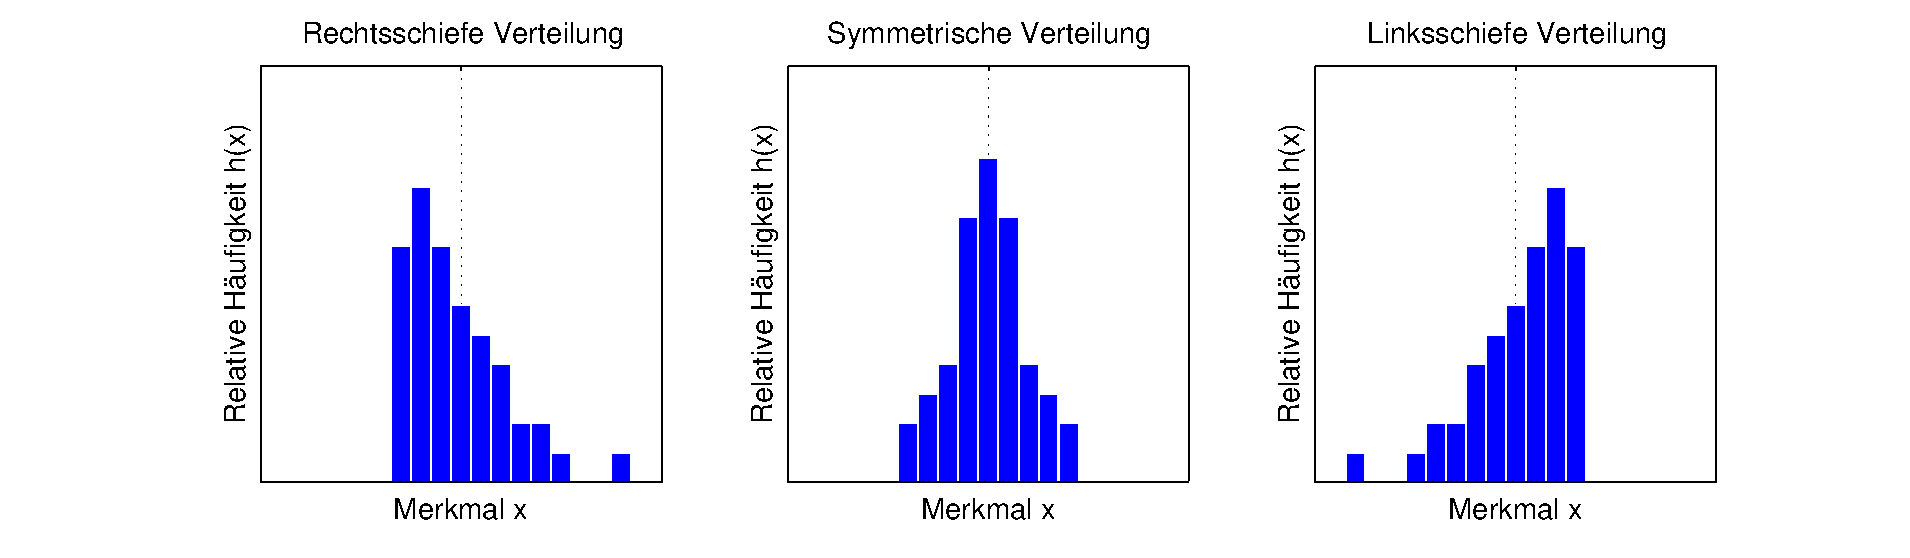
\includegraphics[width=1\textwidth]{Kapitel3/Bilder/image10}}
  \caption{Darstellung von Stichprobenverteilungen mit gleichem Mittelwert und unterschiedlicher Schiefe}
  \label{fig:DefinitionSchiefe}
\end{figure}

\noindent Die Schiefe kann mit zwei unterschiedlichen Kenngr\"{o}{\ss}en charakterisiert werden, dem Momentenkoeffizient und dem Quantilkoeffizient der Schiefe.

\clearpage

{\fontfamily{phv}\selectfont
\noindent\textbf{Momentenkoeffizient der Schiefe}}

\noindent In Analogie an die Varianz $s^{2}$ wird ein Momentenkoeffizient der Schiefe definiert.

\begin{equation}\label{eq:threefourtynine}
g_{M} =\dfrac{N}{(N-1)\cdot (N-2)} \cdot \sum _{n=1}^{N}(\dfrac{x_{n} -\bar{x}}{s} ) ^{3} 
\end{equation} 

\noindent Durch die dritte Potenz der Abweichung der Stichprobenwerte vom Mittelwert bleiben im Vergleich zur Standardabweichung die Vorzeichen bei den Abweichungen erhalten. Bei rechtsschiefen Verteilungen \"{u}berwiegen positive Abweichungen, sodass der Momentenkoeffizient $g_{M}$ positiv wird. Bei linksschiefen Verteilungen weist er entsprechend negative Werte auf. Wegen der Division durch die dritte Potenz der Standardabweichung ist der Momentenkoeffizient der Schiefe dimensionslos und unabh\"{a}ngig von der Messgr\"{o}{\ss}e. F\"{u}r den Fall von in Klassen aufgeteilten Daten errechnet sich der Momentenkoeffizient der Schiefe aus

\begin{equation}\label{eq:threefifty}
g_{M} =\dfrac{\dfrac{1}{N} \cdot \sum _{n=1}^{N}\left(h_{a} (c_{n} )\cdot (c_{n} -\bar{x})^{3} \right) }{s^{3} }
\end{equation} 

\noindent Positive Werte f\"{u}r den Momentenkoeffizienten der Schiefe weisen auf rechtsschiefe Verteilungen, negative Werte weisen auf linksschiefe Verteilungen hin. Ist der Momentenkoeffizient der Schiefe nahe null, handelt es sich um eine symmetrische Verteilung.

\begin{table}[H]
\setlength{\arrayrulewidth}{.1em}
\caption{Bewertung des Momentenkoeffizienten der Schiefe $g_{M}$}
\setlength{\fboxsep}{0pt}%
\colorbox{lightgray}{%
\arrayrulecolor{white}%
\begin{tabular}{| c | c |}
\hline
\parbox[c][0.3in][c]{3.3in}{\smallskip\centering\textbf{\fontfamily{phv}\selectfont{Kennwert}}} & 
\parbox[c][0.3in][c]{3.3in}{\smallskip\centering\textbf{\fontfamily{phv}\selectfont{Symmetrieeigenschaft}}}\\ \hline

\parbox[c][0.3in][c]{3.3in}{\centering\fontfamily{phv}\selectfont{$g_{M}\mathrm{>} 0$}} & 
\parbox[c][0.3in][c]{3.3in}{\centering\fontfamily{phv}\selectfont{tRechtsschiefe Verteilung}}\\ \hline

\parbox[c][0.3in][c]{3.3in}{\centering\fontfamily{phv}\selectfont{$g_{M} = 0$}} & 
\parbox[c][0.3in][c]{3.3in}{\centering\fontfamily{phv}\selectfont{Symmetrische Verteilung}}\\ \hline

\parbox[c][0.3in][c]{3.3in}{\centering\fontfamily{phv}\selectfont{$g_{M} \mathrm{<} 0$}} & 
\parbox[c][0.3in][c]{3.3in}{\centering\fontfamily{phv}\selectfont{Linksschiefe Verteilung}}\\ \hline

\end{tabular}%
}
\label{tab:threefifteen}
\end{table}

\noindent Nachteil des Momentenkoeffizienten der Schiefe ist die durch seine Definition gegebene Abh\"{a}ngigkeit gegen\"{u}ber Ausrei{\ss}ern. Der Befehl zur Berechnung der Schiefe in MATLAB ist in Tabelle \ref{tab:threesixteen} aufgef\"{u}hrt.

\begin{table}[H]
\setlength{\arrayrulewidth}{.1em}
\caption{Berechnung der Symmetriekennwerte von Stichproben in MATLAB}
\setlength{\fboxsep}{0pt}%
\colorbox{lightgray}{%
\arrayrulecolor{white}%
\begin{tabular}{| c | c |}
\hline
\parbox[c][0.3in][c]{3.3in}{\smallskip\centering\textbf{\fontfamily{phv}\selectfont{Symmetriekennwert}}} & 
\parbox[c][0.3in][c]{3.3in}{\smallskip\centering\textbf{\fontfamily{phv}\selectfont{MATLAB-Befehl}}}\\ \hline

\parbox[c][0.3in][c]{3.3in}{\centering\fontfamily{phv}\selectfont{Momentenkoeffizientder Schiefe}} & 
\parbox[c][0.3in][c]{3.3in}{\centering\fontfamily{phv}\selectfont{Rechtsschiefe skewness(x)}}\\ \hline

\end{tabular}%
}
\label{tab:threesixteen}
\end{table}

\noindent Tabelle \ref{tab:threeseventeen} zeigt den Befehl zur Berechnung der Schiefe in Python.

\begin{table}[H]
\setlength{\arrayrulewidth}{.1em}
\caption{Berechnung der Symmetriekennwerte von Stichproben in Python}
\setlength{\fboxsep}{0pt}%
\colorbox{lightgray}{%
\arrayrulecolor{white}%
\begin{tabular}{| c | c |}
\hline
\parbox[c][0.3in][c]{3.3in}{\smallskip\centering\textbf{\fontfamily{phv}\selectfont{Symmetriekennwert}}} & 
\parbox[c][0.3in][c]{3.3in}{\smallskip\centering\textbf{\fontfamily{phv}\selectfont{Python-Befehl}}}\\ \hline

\parbox[c][0.3in][c]{3.3in}{\centering\fontfamily{phv}\selectfont{Momentenkoeffizientder Schiefe}} & 
\parbox[c][0.3in][c]{3.3in}{\centering\fontfamily{phv}\selectfont{scipy.stats.skew}}\\ \hline

\end{tabular}%
}
\label{tab:threeseventeen}
\end{table}

\clearpage 

{\fontfamily{phv}\selectfont
\noindent\textbf{Quantilkoeffizient der Schiefe}}

\noindent Die Symmetrie oder Schiefe einer Verteilung kann \"{u}ber eine Kenngr\"{o}{\ss}e bewertet werden, die die Symmetrie der Quantile einer Stichprobe bewertet. Dazu wird der Quantilkoeffizient der Schiefe berechnet aus

\begin{equation}\label{eq:threefiftyone}
g_{P} =\dfrac{(x_{1-P} -x_{MED})-(x_{MED} -x_{P})}{x_{1-P} -x_{P}}
\end{equation} 

\noindent Der Quantilkoeffizient mit P = 25 \% wird als Quartilkoeffizient der Schiefe bezeichnet. Er ergibt sich zu

\begin{equation}\label{eq:threefiftytwo}
g_{0.25} =\dfrac{(x_{0.75} -x_{MED})-(x_{MED} -x_{0.25})}{x_{0.75} -x_{0.25}}
\end{equation} 

\noindent Die Quartilkoeffizienten bewerten im Z\"{a}hler den Unterschied zwischen der Entfernung des 25\%- beziehungsweise 75\%-Quartils zum Median. Bei symmetrischen Verteilungen ist der Abstand gleich gro{\ss}, der Unterschied ist null. Damit gilt f\"{u}r symmetrische Verteilungen 

\begin{equation}\label{eq:threefiftythree}
g_{0.25} =0
\end{equation} 

\noindent Mit steigender Asymmetrie steigt der Betrag des Quartilkoeffizienten. F\"{u}r die Bewertung gilt die gleiche Klassifizierung wie bei dem Momentenkoeffizient der Schiefe. Positive Quartilkoeffizienten weisen auf eine rechtsschiefe, negative Quartilkoeffizienten weisen auf eine linksschiefe Verteilung hin. Durch den Nenner wird der Quartilkoeffizient so normiert, dass er nur Zahlenwerte im Bereich  $- 1 \leq g_{P} \leq 1$ annehmen kann. Der Quartilkoeffizient reagiert weniger sensitiv auf Ausrei{\ss}er, da dessen Definition mithilfe der Quartile erfolgt. F\"{u}r das Beispiel aus Bild \ref{fig:DefinitionSchiefe} ergeben sich die in Tabelle \ref{tab:threeeightteen} dargestellten Koeffizienten.

\begin{table}[H]
\setlength{\arrayrulewidth}{.1em}
\caption{Charakterisierung der Schiefe f\"{u}r die Stichprobe aus Bild \ref{fig:DefinitionSchiefe}}
\setlength{\fboxsep}{0pt}%
\colorbox{lightgray}{%
\arrayrulecolor{white}%
\begin{tabular}{| c | c | c | c |}
\hline
\parbox[c][0.6in][c]{1.55in}{\smallskip\centering\textbf{\fontfamily{phv}\selectfont{Bild 3.10}}} & 
\parbox[c][0.6in][c]{1.55in}{\smallskip\centering\textbf{\fontfamily{phv}\selectfont{Momentenkoeffizient der Schiefe g$_{\mathbf{M}}$}}} & 
\parbox[c][0.6in][c]{1.55in}{\smallskip\centering\textbf{\fontfamily{phv}\selectfont{Quartilkoeffizient der Schiefe g$_{\mathbf{P}}$}}} & 
\parbox[c][0.6in][c]{1.55in}{\smallskip\centering\textbf{\fontfamily{phv}\selectfont{Folgerung für die Verteilung}}}\\ \hline

\parbox[c][0.3in][c]{1.55in}{\centering\fontfamily{phv}\selectfont{Links}} & 
\parbox[c][0.3in][c]{1.55in}{\centering\fontfamily{phv}\selectfont{1.1017}} & 
\parbox[c][0.3in][c]{1.55in}{\centering\fontfamily{phv}\selectfont{0.3333}} & 
\parbox[c][0.3in][c]{1.55in}{\centering\fontfamily{phv}\selectfont{Rechtsschief}}\\ \hline

\parbox[c][0.3in][c]{1.55in}{\centering\fontfamily{phv}\selectfont{Mitte}} & 
\parbox[c][0.3in][c]{1.55in}{\centering\fontfamily{phv}\selectfont{0}} & 
\parbox[c][0.3in][c]{1.55in}{\centering\fontfamily{phv}\selectfont{0}} & 
\parbox[c][0.3in][c]{1.55in}{\centering\fontfamily{phv}\selectfont{Symmetrisch}}\\ \hline

\parbox[c][0.3in][c]{1.55in}{\centering\fontfamily{phv}\selectfont{Rechts}} & 
\parbox[c][0.3in][c]{1.55in}{\centering\fontfamily{phv}\selectfont{- 1.1017}} & 
\parbox[c][0.3in][c]{1.55in}{\centering\fontfamily{phv}\selectfont{- 0.3333}} & 
\parbox[c][0.3in][c]{1.55in}{\centering\fontfamily{phv}\selectfont{Linksschief}}\\ \hline

\end{tabular}%
}
\label{tab:threeeightteen}
\end{table}

\noindent Beide Ma{\ss}e f\"{u}r die Schiefe weisen dasselbe Vorzeichen, aber unterschiedliche Zahlenwerte auf und sind deshalb nicht direkt miteinander vergleichbar.


\subsubsection{Lageregeln zur Interpretation der Symmetrie einer Stichprobe}

\noindent Die Symmetrieeigenschaften der H\"{a}ufigkeitsverteilung einer Stichprobe k\"{o}nnen auch an der Lage von Median und Mittelwert abgelesen werden. Die Verteilung der Stichprobe in Bild \ref{fig:DefinitionSchiefe} links f\"{a}llt nach links steil ab und l\"{a}uft nach rechts flach aus, sie ist also rechtsschief. Mittelwert und Median berechnen sich zu 

\begin{equation}\label{eq:threefiftyfour}
\bar{x}=10
\end{equation} 

\noindent und 

\begin{equation}\label{eq:threefiftyfive}
x_{MED} =9.26
\end{equation} 

\noindent F\"{u}r die mittlere H\"{a}ufigkeitsverteilung stimmen Mittelwert und Median \"{u}berein. 

\begin{equation}\label{eq:threefiftysix}
\bar{x}=x_{MED} =10
\end{equation} 

\noindent Die rechte H\"{a}ufigkeitsverteilung ist linksschief, f\"{u}r sie errechnen sich die Lagekennwerte zu

\begin{equation}\label{eq:threefiftyseven}
\bar{x}=10
\end{equation} 

\noindent und

\begin{equation}\label{eq:threefiftyeight}
x_{MED} =10.74
\end{equation} 

\noindent Dieses Ergebnis kann verallgemeinert werden. Tabelle \ref{tab:threenineteen} fasst die Lageregeln zur Beschreibung der Symmetrie einer H\"{a}ufigkeitsverteilung zusammen. Je st\"{a}rker sich die Lagekennwerte voneinander unterscheiden, desto schiefer ist die Verteilung.

\begin{table}[H]
\setlength{\arrayrulewidth}{.1em}
\caption{Lageregeln von Median und arithmetischem Mittelwert zur Beschreibung der Symmetri}
\setlength{\fboxsep}{0pt}%
\colorbox{lightgray}{%
\arrayrulecolor{white}%
\begin{tabular}{| c | c |}
\hline
\parbox[c][0.3in][c]{3.3in}{\smallskip\centering\textbf{\fontfamily{phv}\selectfont{Lagekennwerte}}} & 
\parbox[c][0.3in][c]{3.3in}{\smallskip\centering\textbf{\fontfamily{phv}\selectfont{Symmetrieeigenschaft}}}\\ \hline

\parbox[c][0.3in][c]{3.3in}{\centering\fontfamily{phv}\selectfont{$\bar{x}>x_{MED}$}} & 
\parbox[c][0.3in][c]{3.3in}{\centering\fontfamily{phv}\selectfont{Rechtsschiefe Verteilung}}\\ \hline

\parbox[c][0.3in][c]{3.3in}{\centering\fontfamily{phv}\selectfont{$\bar{x}>x_{MED}$}} & 
\parbox[c][0.3in][c]{3.3in}{\centering\fontfamily{phv}\selectfont{Symmetrische Verteilung}}\\ \hline

\parbox[c][0.3in][c]{3.3in}{\centering\fontfamily{phv}\selectfont{$\bar{x}>x_{MED}$}} & 
\parbox[c][0.3in][c]{3.3in}{\centering\fontfamily{phv}\selectfont{Linksschiefe Verteilung}}\\ \hline

\end{tabular}%
}
\label{tab:threenineteen}
\end{table}

\noindent
\colorbox{lightgray}{%
\arrayrulecolor{white}%
\renewcommand\arraystretch{0.6}%
\begin{tabular}{ wl{16.5cm} }
{\fontfamily{phv}\selectfont
\noindent{Beispiel: Dicke einer Schutzlackbeschichtung}}
\end{tabular}%
}\bigskip

\noindent Als Beispiel f\"{u}r eine schiefe Verteilung soll die Dicke einer Schutzlackbeschichtung betrachtet werden, die von einer Automatisierungseinrichtung auf Platinen aufgebracht wird. Der Sollwert der Schichtdicke ist spezifiziert auf 10 µm. Bei 100 Platinen wurde die aufgetragene Schutzschicht vermessen. Dabei ergab sich die in Tabelle \ref{tab:threetwenty} aufgelistete H\"{a}ufigkeitsverteilung.

\begin{table}[H]
\setlength{\arrayrulewidth}{.1em}
\caption{H\"{a}ufigkeitsverteilung der Stichprobe}
\setlength{\fboxsep}{0pt}%
\colorbox{lightgray}{%
\arrayrulecolor{white}%
\begin{tabular}{| c | c | c | c | c | c |}
\hline
\parbox[c][0.6in][c]{1in}{\smallskip\centering\textbf{\fontfamily{phv}\selectfont{D / µm}}} & 
\parbox[c][0.6in][c]{1in}{\smallskip\centering\textbf{\fontfamily{phv}\selectfont{Anzah H\"{a}ufigkeit h$_{\mathbf{A}}$(D)}}} & 
\parbox[c][0.6in][c]{1in}{\smallskip\centering\textbf{\fontfamily{phv}\selectfont{Relative H\"{a}ufigkeith(D)}}} & 
\parbox[c][0.6in][c]{1in}{\smallskip\centering\textbf{\fontfamily{phv}\selectfont{D / µm}}} & 
\parbox[c][0.6in][c]{1in}{\smallskip\centering\textbf{\fontfamily{phv}\selectfont{Anzahl H\"{a}ufigkeit h$_{\mathbf{A}}$(D)}}} & 
\parbox[c][0.6in][c]{1in}{\smallskip\centering\textbf{\fontfamily{phv}\selectfont{Relative H\"{a}ufigkeith(D)}}}\\ \hline

\parbox[c][0.3in][c]{1in}{\centering\fontfamily{phv}\selectfont{4}} & 
\parbox[c][0.3in][c]{1in}{\centering\fontfamily{phv}\selectfont{13}} &
\parbox[c][0.3in][c]{1in}{\centering\fontfamily{phv}\selectfont{0.13}} & 
\parbox[c][0.3in][c]{1in}{\centering\fontfamily{phv}\selectfont{24}} &
\parbox[c][0.3in][c]{1in}{\centering\fontfamily{phv}\selectfont{5}} & 
\parbox[c][0.3in][c]{1in}{\centering\fontfamily{phv}\selectfont{0.05}}\\ \hline

\parbox[c][0.3in][c]{1in}{\centering\fontfamily{phv}\selectfont{8}} & 
\parbox[c][0.3in][c]{1in}{\centering\fontfamily{phv}\selectfont{33}} &
\parbox[c][0.3in][c]{1in}{\centering\fontfamily{phv}\selectfont{0.33}} & 
\parbox[c][0.3in][c]{1in}{\centering\fontfamily{phv}\selectfont{28}} &
\parbox[c][0.3in][c]{1in}{\centering\fontfamily{phv}\selectfont{2}} & 
\parbox[c][0.3in][c]{1in}{\centering\fontfamily{phv}\selectfont{0.02}}\\ \hline

\parbox[c][0.3in][c]{1in}{\centering\fontfamily{phv}\selectfont{12}} & 
\parbox[c][0.3in][c]{1in}{\centering\fontfamily{phv}\selectfont{21}} &
\parbox[c][0.3in][c]{1in}{\centering\fontfamily{phv}\selectfont{0.21}} & 
\parbox[c][0.3in][c]{1in}{\centering\fontfamily{phv}\selectfont{32}} &
\parbox[c][0.3in][c]{1in}{\centering\fontfamily{phv}\selectfont{2}} & 
\parbox[c][0.3in][c]{1in}{\centering\fontfamily{phv}\selectfont{0.02}}\\ \hline

\parbox[c][0.3in][c]{1in}{\centering\fontfamily{phv}\selectfont{16}} & 
\parbox[c][0.3in][c]{1in}{\centering\fontfamily{phv}\selectfont{16}} &
\parbox[c][0.3in][c]{1in}{\centering\fontfamily{phv}\selectfont{0.16}} & 
\parbox[c][0.3in][c]{1in}{\centering\fontfamily{phv}\selectfont{36}} &
\parbox[c][0.3in][c]{1in}{\centering\fontfamily{phv}\selectfont{0}} & 
\parbox[c][0.3in][c]{1in}{\centering\fontfamily{phv}\selectfont{0.00}}\\ \hline

\parbox[c][0.3in][c]{1in}{\centering\fontfamily{phv}\selectfont{20}} & 
\parbox[c][0.3in][c]{1in}{\centering\fontfamily{phv}\selectfont{7}} &
\parbox[c][0.3in][c]{1in}{\centering\fontfamily{phv}\selectfont{0.07}} & 
\parbox[c][0.3in][c]{1in}{\centering\fontfamily{phv}\selectfont{40}} &
\parbox[c][0.3in][c]{1in}{\centering\fontfamily{phv}\selectfont{1}} & 
\parbox[c][0.3in][c]{1in}{\centering\fontfamily{phv}\selectfont{0.01}}\\ \hline

\end{tabular}%
}
\label{tab:threetwenty}
\end{table}

\clearpage

\noindent In Bild \ref{fig:Schichtdicke} ist zu erkennen, dass die Verteilung nach links wesentlich steiler abf\"{a}llt als nach rechts. Es handelt sich daher um eine rechtsschiefe Verteilung.

\noindent 
\begin{figure}[H]
  \centerline{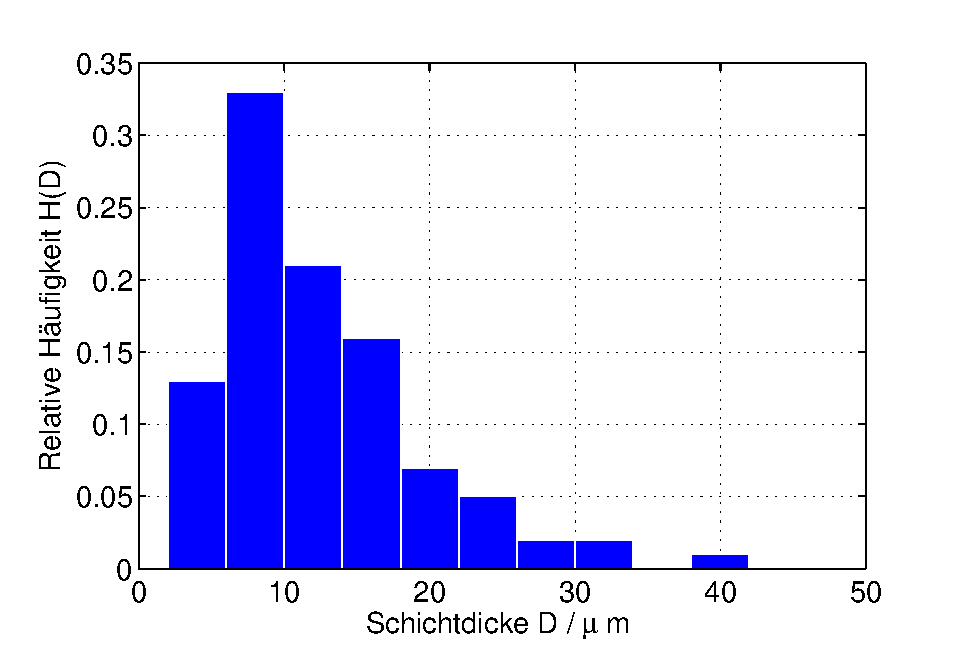
\includegraphics[width=0.5\textwidth]{Kapitel3/Bilder/image11}}
  \caption{Relative H\"{a}ufigkeitsverteilung der Lackdicke}
  \label{fig:Schichtdicke}
\end{figure}

\noindent Der Momentenkoeffizient der Schiefe berechnet sich f\"{u}r das Beispiel der Schichtdicken mit der Standardabweichung

\begin{equation}\label{eq:threefiftynine}
s=\sqrt{\dfrac{1}{N-1} \cdot \sum _{n=1}^{N}\left(h_{A} (c_{n})\cdot (c_{n} -\bar{D})^{2} \right)} =7.007 \mu m
\end{equation} 

\noindent zu

\begin{equation}\label{eq:threesixty}
g_{M} =\dfrac{\dfrac{1}{N} \cdot \sum _{n=1}^{N}\left(h_{A} (c_{n})\cdot (c_{n} -\bar{D})^{3} \right)}{s^{3}} =1.3
\end{equation} 

\noindent Wegen des positiven Vorzeichens des Momentenkoeffizienten handelt es sich um eine rechtsschiefe Verteilung, was die Einsch\"{a}tzung anhand Bild \ref{fig:Schichtdicke} best\"{a}tigt. F\"{u}r die Berechnung des 25\%-Quartilkoeffizienten der Schiefe werden die Quartile der Verteilung ben\"{o}tigt. Sie berechnen sich aus den angegebenen Klassen zu

\begin{equation}\label{eq:threesixtyone}
D_{0.25} =c_{n-1} +\dfrac{d\cdot \left(0.25-H(c_{n-1})\right)}{h(c_{n})} =4 \mu m+\dfrac{4 \mu m\cdot (0.25-0.13)}{0.33} =5.455 \mu m
\end{equation} 

\begin{equation}\label{eq:threesixtytwo}
D_{0.5} =D_{MED} =c_{n-1} +\dfrac{d\cdot (0.5-H\left(c_{n-1})\right)}{h(c_{n})} =8 \mu m+\dfrac{4 \mu m\cdot (0.5-0.46)}{0.21} =8.763 \mu m
\end{equation} 

\noindent und

\begin{equation}\label{eq:threesixtythree}
D_{0.75} =c_{n-1} +\dfrac{d\cdot \left(0.75-H(c_{n-1})\right)}{h(c_{n})} =12 \mu m+\dfrac{4 \mu m\cdot (0.75-0.67)}{0.16} =14 \mu m
\end{equation} 

\noindent Der 25\%-Quartilkoeffizient der Schiefe folgt damit nach Gleichung \eqref{eq:threesixtyone} zu

\begin{equation}\label{eq:threesixtyfour}
g_{0.25} =\dfrac{(D_{0.75} -D_{0.5})-(D_{0.5} -D_{0.25})}{D_{0.75} -D_{0.25} } =\dfrac{(14-8.763)-(8.763-5.455)}{14-5.455} = 0.2259
\end{equation} 

\noindent Das positive Vorzeichen des 25\%-Quartilkoeffizienten weist auf eine rechtsschiefe Verteilung hin und best\"{a}tigt damit das Ergebnis des Momentenkoeffizienten der Schiefe und der grafischen Beurteilung. Zus\"{a}tzlich kann die Lage des arithmetischen Mittelwertes 

\begin{equation}\label{eq:threesixtyfive}
\bar{D}=\sum _{n=1}^{N}\left(D_{n} \cdot h(c_{n})\right) =12.44 \mu m
\end{equation} 

\noindent in Relation zum Median zur Bewertung der Schiefe nach Tabelle \ref{tab:threenineteen} ausgewertet werden. Auch nach diesem Kriterium ist die Stichprobe rechtsschief. Alle Bewertungsm\"{o}glichkeiten der Schiefe f\"{u}hren damit zum gleichen Ergebnis.\newline

\noindent Schiefe oder asymmetrische H\"{a}ufigkeitsverteilungen treten insbesondere dann auf, wenn das untersuchte Merkmal durch einen nat\"{u}rlichen einseitigen Grenzwert eingeschr\"{a}nkt wird. Im vorigen Beispiel der Dicke einer Schutzlackschicht wird die H\"{a}ufigkeitsverteilung nach links begrenzt, da die Schichtdicke nie kleiner als null werden kann. Weitere Beispiele w\"{a}ren die Rauheit einer Oberfl\"{a}che oder der Durchmesser einer Bohrung, der durch den Durchmesser des verwendeten Bohrers nach unten begrenzt ist. In Kapitel 4 wird sich zeigen, dass asymmetrische Verteilungen auch zur Absch\"{a}tzung von Lebensdauern oder Ausfallzeiten herangezogen werden. 


\subsubsection{Box-Plot}

\noindent In den Abschnitten \ref{threethreeone} und \ref{threethreetwo} werden Kenngr\"{o}{\ss}en f\"{u}r die numerische Beschreibung von Stichproben und die Charakterisierung von Verteilungen vorgestellt. Die wesentlichen Gr\"{o}{\ss}en k\"{o}nnen aus dem sogenannten Box-Plot abgelesen werden, der im Folgenden vorgestellt wird. Der Box-Plot fasst f\"{u}nf charakteristische Punkte einer Verteilung zusammen:

\begin{itemize}
    \item Minimaler Stichprobenwert x$_{MIN}$
    \item 25\%-Quartil x$_{0.25}$
    \item Median x$_{MED}$
    \item 75\%-Quartil x$_{0.75}$
    \item Maximaler Stichprobenwert x$_{MAX}$
\end{itemize}

\noindent Die Idee des Box-Plots ist in Bild \ref{fig:Box-Plots} dargestellt. Anfang und Ende der Box stellen die 25\%- und 75\%-Quartile dar. Die L\"{a}nge der Box repr\"{a}sentiert damit den Interquartilabstand. Der Median wird als Balken in der Box eingezeichnet. Zwei Linien au{\ss}erhalb der Box, die sogenannten Whisker, zeigen die minimalen und maximalen Werte x${}_{MIN}$ und x${}_{MAX}$ der Stichprobe. Ausrei{\ss}er werden nicht zur Bestimmung des minimalen und maximalen Wertes verwendet. Als Ausrei{\ss}er gelten Werte, die erheblich kleiner als das 25\%-Quartil und erheblich gr\"{o}{\ss}er als das 75\%-Quartil sind. Mathematisch wird diese Aussage durch die Bedingungen 

\begin{equation}\label{eq:threesixtysix}
x_{OUT} <x_{0.25} -1.5\cdot (x_{0.75} -x_{0.25})
\end{equation}

beziehungsweise 

\begin{equation}\label{eq:threesixtyseven}
x_{OUT} >x_{0.75} +1.5\cdot (x_{0.75} -x_{0.25})
\end{equation}

\noindent formuliert. Ausrei{\ss}er werden als separates Kreuz dargestellt. 

\clearpage

\noindent 
\begin{figure}[H]
  \centerline{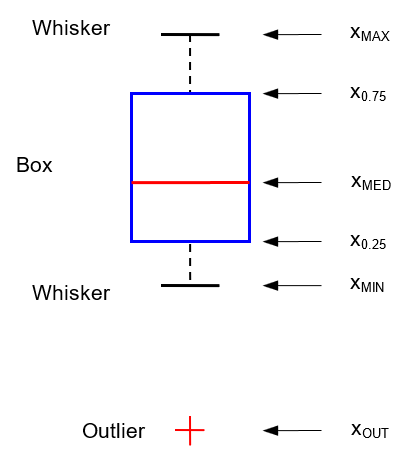
\includegraphics[width=0.5\textwidth]{Kapitel3/Bilder/image12}}
  \caption{Grundidee des Box-Plots}
  \label{fig:Box-Plots}
\end{figure}

\noindent Neben der grafischen Darstellung eignet sich der Box-Plot f\"{u}r eine Interpretation der Stichprobenkennwerte. 

\noindent Bild \ref{fig:DefinitionSchiefeBoxPlot} stellt als Beispiel den Box-Plot f\"{u}r die Stichproben aus Bild \ref{fig:DefinitionSchiefe} dar. Die unsymmetrische Lage des Median in der Box weist auf eine unsymmetrische Stichprobe hin.

\noindent 
\begin{figure}[H]
  \centerline{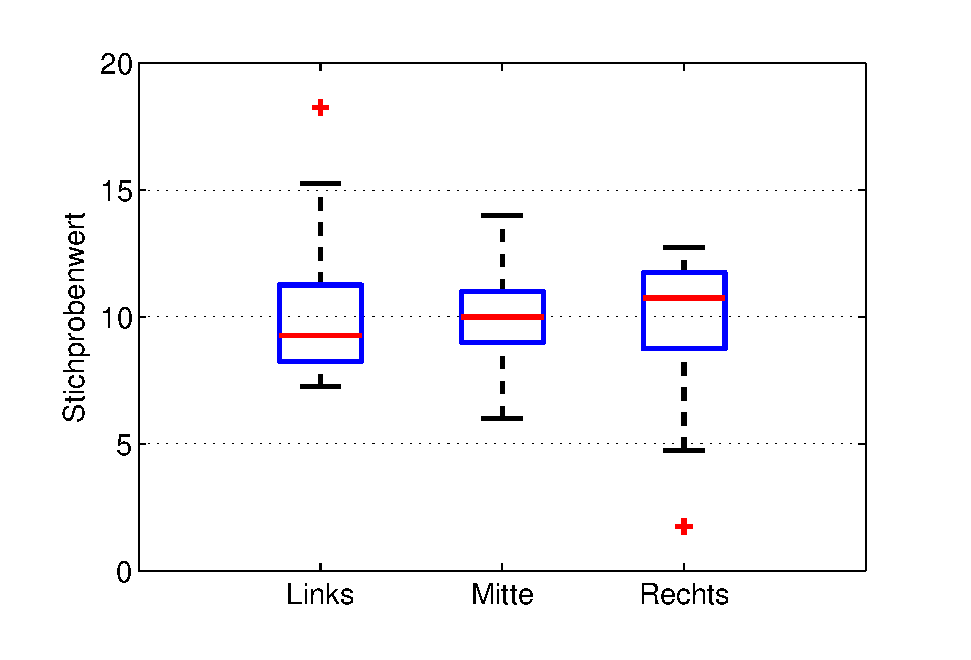
\includegraphics[width=0.5\textwidth]{Kapitel3/Bilder/image13}}
  \caption{Box-Plot f\"{u}r die Stichproben aus \ref{fig:DefinitionSchiefe}}
  \label{fig:DefinitionSchiefeBoxPlot}
\end{figure}

\noindent MATLAB und python Python bieten zur Erstellung eines Box-Plots eine separate Funktion an.

\begin{table}[H]
\setlength{\arrayrulewidth}{.1em}
\caption{Darstellung des Box-Plots einer Stichprobe in MATLAB}
\setlength{\fboxsep}{0pt}%
\colorbox{lightgray}{%
\arrayrulecolor{white}%
\begin{tabular}{| c | c |}
\hline
\parbox[c][0.3in][c]{3.3in}{\smallskip\centering\textbf{\fontfamily{phv}\selectfont{Darstellung}}} & 
\parbox[c][0.3in][c]{3.3in}{\smallskip\centering\textbf{\fontfamily{phv}\selectfont{MATLAB-Befehl}}}\\ \hline

\parbox[c][0.3in][c]{3.3in}{\centering\fontfamily{phv}\selectfont{Box-Plot}} & 
\parbox[c][0.3in][c]{3.3in}{\centering\fontfamily{phv}\selectfont{boxplot(x)}}\\ \hline

\end{tabular}%
}
\label{tab:threetwentyone}
\end{table}

\begin{table}[H]
\setlength{\arrayrulewidth}{.1em}
\caption{Darstellung des Box-Plots einer Stichprobe in Python}
\setlength{\fboxsep}{0pt}%
\colorbox{lightgray}{%
\arrayrulecolor{white}%
\begin{tabular}{| c | c |}
\hline
\parbox[c][0.3in][c]{3.3in}{\smallskip\centering\textbf{\fontfamily{phv}\selectfont{Darstellung}}} & 
\parbox[c][0.3in][c]{3.3in}{\smallskip\centering\textbf{\fontfamily{phv}\selectfont{MATLAB-Befehl}}}\\ \hline

\parbox[c][0.3in][c]{3.3in}{\centering\fontfamily{phv}\selectfont{Box-Plot}} & 
\parbox[c][0.3in][c]{3.3in}{\centering\fontfamily{phv}\selectfont{matplotlib.pyplot.boxplot}}\\ \hline

\end{tabular}%
}
\label{tab:threetwentytwo}
\end{table}

\clearpage

\subsection{Anwendungsbeispiel: Charakterisierung eines Klebeprozesses}

\noindent Eine Automatisierungseinrichtung hat zum Befestigen einer Folie im Automobilbau Klebermengen dosiert. Die in Tabelle 3.23Tabelle 3.23 enthaltenen Zahlenwerte stellen eine Stichprobe mit einem Umfang von N = 40 abgef\"{u}llten Klebermengen dar. 

\begin{table}[H]
\setlength{\arrayrulewidth}{.1em}
\caption{Stichprobenwerte zur Bewertung eines Klebeprozesses}
\setlength{\fboxsep}{0pt}%
\colorbox{lightgray}{%
\arrayrulecolor{white}%
\begin{tabular}{| wc{4cm} | wc{2cm} | wc{2cm} | wc{2cm} | wc{2cm} | wc{2cm} }
\hline\xrowht{15pt}

\fontfamily{phv}\selectfont\textbf{Messung} & \multicolumn{5}{c}{\fontfamily{phv}\selectfont\textbf{Messwerte Klebermenge m / mg}} \\ \hline \xrowht{15pt}

\fontfamily{phv}\selectfont\textbf{1 - 5} &
50.18 & 51.85 & 51.09 & 50.09 & 51.03\\ \hline\xrowht{15pt}

\fontfamily{phv}\selectfont\textbf{6 - 10} & 
50.69 & 51.76 & 51.23 & 51.49 & 51.62\\ \hline\xrowht{15pt}

\fontfamily{phv}\selectfont\textbf{11- 15} &
50.52 & 51.33 & 51.18 & 51.76 & 52.62\\ \hline\xrowht{15pt}

\fontfamily{phv}\selectfont\textbf{16 - 20} &
51.49 & 51.19 & 51.28 & 50.82 & 50.01\\ \hline\xrowht{15pt}

\fontfamily{phv}\selectfont\textbf{21 - 25} &
51.6 & 50.94 & 51.54 & 51.3 & 50.91\\ \hline\xrowht{15pt}

\fontfamily{phv}\selectfont\textbf{26 - 30} &
51.44 & 51.78 & 51.37 & 51.36 & 50.54\\ \hline\xrowht{15pt}

\fontfamily{phv}\selectfont\textbf{31 - 35} &
52.2 & 52.12 & 49.4 & 49.76 & 51.54\\ \hline\xrowht{15pt}

\fontfamily{phv}\selectfont\textbf{36 - 40} &
50.64 & 50.37 & 50.16 & 50.61 & 50.38\\ \hline 

\end{tabular}%
}
\label{tab:threetwentythree}
\end{table}

\noindent Der Datensatz wird im Folgenden ohne Aufteilung der Daten in Klassen und mit Aufteilung der Daten in Klassen ausgewertet. Abschlie{\ss}end werden die Ergebnisse miteinander verglichen.


\subsubsection{Datenanalyse in MATLAB ohne Aufteilung der Daten in Klassen}

\noindent Bei dem untersuchten Klebeprozess handelt es sich um einen kontinuierlichen Prozess, jeder Messwert besitzt hierbei die absolute H\"{a}ufigkeit 1. Eine Darstellung als H\"{a}ufigkeitsverteilung l\"{a}sst somit keine R\"{u}ckschl\"{u}sse auf den zu untersuchenden Prozess zu. Deshalb werden die Daten mit einem Streudiagramm und der relativen Summenh\"{a}ufigkeit beschrieben.

\begin{figure}[H]
  \centerline{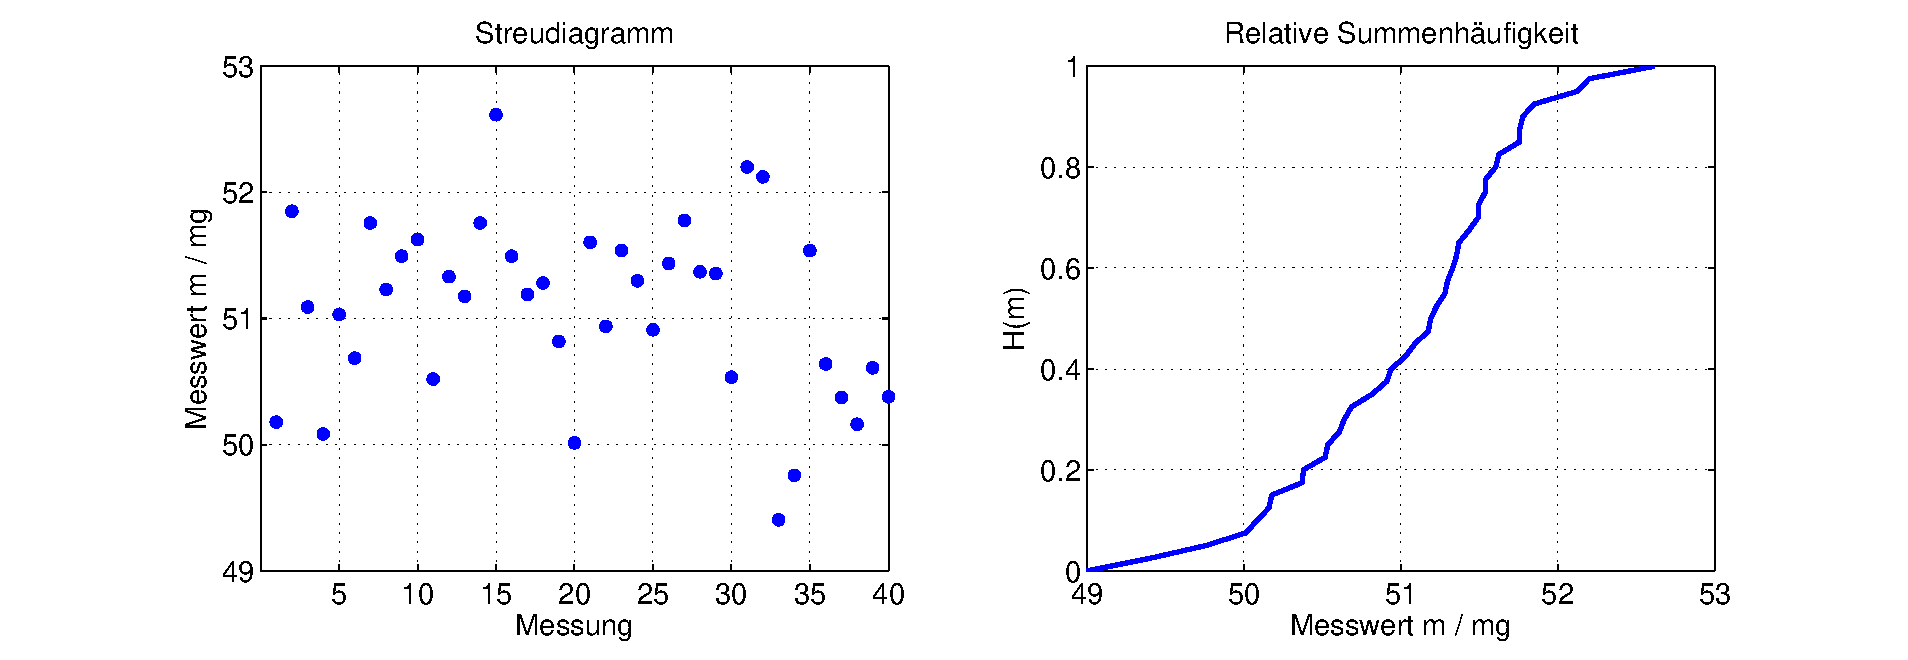
\includegraphics[width=1\textwidth]{Kapitel3/Bilder/image14}}
  \caption{Darstellung der Messwerte als Streudiagramm und als relative Summenh\"{a}ufigkeit}
  \label{fig:Streudiagramm}
\end{figure}

\noindent Im Streudiagramm in Bild \ref{fig:Streudiagramm} ist zu erkennen, dass sich die Messwerte in einem Bereich von 49 bis 53 mg befinden. In der Darstellung der relativen Summenh\"{a}ufigkeit kann abgelesen werden, dass der Median mit einer relativen Summenh\"{a}ufigkeit von 0.5 bei einer Klebemenge von 51.25 mg liegt. Die Grafik wurde mit dem folgenden MATLAB-Code erzeugt.

\clearpage

\lstinputlisting[caption = {}]{Kapitel3/mat1.m}

\noindent Um die Lage der Messwerte genauer zu beschreiben, werden die in Abschnitt 3.3.1 eingef\"{u}hrten Lagekennwerte berechnet. F\"{u}r die Messwerte aus Tabelle \ref{tab:threetwentythree} ergibt sich der arithmetische Mittelwert zu

\begin{equation}\label{eq:threesixtyeight}
\bar{m}=\dfrac{1}{N} \cdot \sum _{n=1}^{N}m_{n}  =51.08 mg
\end{equation}

\noindent Der Median wird nach Sortieren der Messwerte aus dem Mittelwert der beiden mittleren Messwerte bestimmt.

\begin{equation}\label{eq:threesixtynine}
m_{MED} =\dfrac{m_{17} +m_{8} }{2} =\dfrac{51.19 mg + 51.23 mg}{2} =51.21mg
\end{equation}

\noindent Zus\"{a}tzlich zu den Kennwerten zur Beschreibung der Lage werden in Abschnitt 3.3.2 Streuungskennwerte definiert. Die Varianz der Messwerte berechnet sich zu

\begin{equation}\label{eq:threeseventy}
s^{2} =\dfrac{1}{N-1} \cdot \sum _{n=1}^{N}\left(m_{n} -\bar{m}\right)^{2}  =  0.49 mg^{2}
\end{equation}

\noindent Aus der Wurzel der Varianz folgt die Standardabweichung von

\begin{equation}\label{eq:threeseventyone}
s=\sqrt{s^{2}} = 0.70 mg
\end{equation}

\noindent Der Interquartilabstand ergibt sich aus der Differenz des 75\%-Quartils und des 25\%-Quartils der Messwerte zu

\begin{equation}\label{eq:threeseventytwo}
IQR=m_{0.75} -m_{0.25} =50.57 mg-51.54 mg= 0.97 mg
\end{equation}

\clearpage 

\noindent Der verwendete Programmcode zur Berechnung der Lage- und Streuungskennwerte mithilfe von MATLAB ist im Folgenden dargestellt.

\lstinputlisting[caption = {}]{Kapitel3/mat2.m}

\noindent Da aus Bild \ref{fig:DefinitionSchiefeBoxPlot2} keine Aussage hinsichtlich der Schiefe der Verteilung gemacht werden kann, wird der 25\%-Quartilkoeffizient und der Momentenkoeffizient der Schiefe zur Bewertung herangezogen. Der 25\%-Quartilkoeffizient der Schiefe berechnet sich zu

\begin{equation}\label{eq:threeseventythree}
g_{0.25} =\dfrac{\left(m_{0.75} -m_{MED} \right)-\left(m_{MED} -m_{0.25} \right)}{m_{0.75} -m_{0.25}} =\dfrac{\left(51.54-51.21\right)-\left(51.21-50.57\right)}{51.54-50.57} =-0.32
\end{equation}

\noindent und der Momentenkoeffizient der Schiefe folgt zu

\begin{equation}\label{eq:threeseventyfour}
g_{M} =\dfrac{\dfrac{1}{N} \cdot \displaystyle\sum\limits _{n=1}^{N}\left(m_{n} -\bar{m}\right)^{3}}{s^{3}} =-0.28
\end{equation}

\noindent Beide Werte weisen auf eine linksschiefe Verteilung hin. Die Berechnung der Kennwerte der Schiefe wird mit MATLAB mit der folgenden Befehlssequenz durchgef\"{u}hrt

\lstinputlisting[caption = {}]{Kapitel3/mat3.m}

\noindent Der Klebeprozess wird mit den Stichprobenwerten aus Tabelle \ref{tab:threetwentythree} sowohl grafisch dargestellt als auch durch Kennwerte beschrieben. Dabei werden die Daten nicht in Klassen eingeteilt. Um den Unterschied zu zeigen, wird auf Basis der gleichen Stichprobenwerte nun eine Datenanalyse durchgef\"{u}hrt, bei der die Messwerte in Klassen eingeteilt werden.


\subsubsection{Datenanalyse in MATLAB mit Aufteilung der Daten in Klassen}

\noindent Zun\"{a}chst muss f\"{u}r die Daten eine sinnvolle Klasseneinteilung gefunden werden. Hierbei wird insbesondere darauf geachtet, dass die Klassenmitten m\"{o}glichst Zahlen mit wenig Nachkommastellen sind. Bei dem Datensatz aus Tabelle \ref{tab:threetwentythree} mit einem Minimalwert von m$_{MIN}$ = 49.40 mg und einem Maximalwert von m$_{MAX}$ = 52.62 mg bietet es sich an, eine Klassenbreite d von 1 mg zu w\"{a}hlen. Die Messwerte lassen sich damit in 5 Klassen einteilen, die in Tabelle \ref{tab:threetwentyfour} zusammen mit ihrer absoluten und ihrer relativen H\"{a}ufigkeit angegeben sind.

\clearpage

\begin{table}[H]
\setlength{\arrayrulewidth}{.1em}
\caption{Stichprobenwerte zur \"{U}berpr\"{u}fung eines Klebeprozesses eingeteilt in Klassen}
\setlength{\fboxsep}{0pt}%
\colorbox{lightgray}{%
\arrayrulecolor{white}%
\begin{tabular}{| c | c | c | c | c |}
\hline
\parbox[c][0.6in][c]{1.2in}{\smallskip\centering\textbf{\fontfamily{phv}\selectfont{c / mg}}} & 
\parbox[c][0.6in][c]{1.2in}{\smallskip\centering\textbf{\fontfamily{phv}\selectfont{Anzahl Häufigkeit h$_{\mathbf{A}}$(c)}}} & 
\parbox[c][0.6in][c]{1.2in}{\smallskip\centering\textbf{\fontfamily{phv}\selectfont{Relative Häufigkeit h(c)}}} & 
\parbox[c][0.6in][c]{1.2in}{\smallskip\centering\textbf{\fontfamily{phv}\selectfont{Absolute Summenhäufigkeit H$_{\mathbf{A}}$(c)}}} & 
\parbox[c][0.6in][c]{1.2in}{\smallskip\centering\textbf{\fontfamily{phv}\selectfont{Relative Summenhäufigkeit H(c)}}}\\ \hline

\parbox[c][0.3in][c]{1.2in}{\centering\textbf{49}} & 
\parbox[c][0.3in][c]{1.2in}{\centering{1}} & 
\parbox[c][0.3in][c]{1.2in}{\centering{0.025}} & 
\parbox[c][0.3in][c]{1.2in}{\centering{1}} & 
\parbox[c][0.3in][c]{1.2in}{\centering{0.025}}\\ \hline

\parbox[c][0.3in][c]{1.2in}{\centering\textbf{50}} & 
\parbox[c][0.3in][c]{1.2in}{\centering{7}} & 
\parbox[c][0.3in][c]{1.2in}{\centering{0.175}} & 
\parbox[c][0.3in][c]{1.2in}{\centering{8}} & 
\parbox[c][0.3in][c]{1.2in}{\centering{0.2}}\\ \hline

\parbox[c][0.3in][c]{1.2in}{\centering\textbf{51}} & 
\parbox[c][0.3in][c]{1.2in}{\centering{21}} & 
\parbox[c][0.3in][c]{1.2in}{\centering{0.525}} & 
\parbox[c][0.3in][c]{1.2in}{\centering{29}} & 
\parbox[c][0.3in][c]{1.2in}{\centering{0.725}}\\ \hline

\parbox[c][0.3in][c]{1.2in}{\centering\textbf{52}} & 
\parbox[c][0.3in][c]{1.2in}{\centering{10}} & 
\parbox[c][0.3in][c]{1.2in}{\centering{0.25}} & 
\parbox[c][0.3in][c]{1.2in}{\centering{39}} & 
\parbox[c][0.3in][c]{1.2in}{\centering{0.975}}\\ \hline

\parbox[c][0.3in][c]{1.2in}{\centering\textbf{53}} & 
\parbox[c][0.3in][c]{1.2in}{\centering{1}} & 
\parbox[c][0.3in][c]{1.2in}{\centering{0.025}} & 
\parbox[c][0.3in][c]{1.2in}{\centering{40}} & 
\parbox[c][0.3in][c]{1.2in}{\centering{1}}\\ \hline

\end{tabular}%
}
\label{tab:threetwentyfour}
\end{table}

\noindent Die relative H\"{a}ufigkeit und die relative Summenh\"{a}ufigkeit der in Klassen eingeteilten Stichprobenwerte sind in Bild \ref{fig:DefinitionSchiefeBoxPlot2} dargestellt.

\noindent 
\begin{figure}[H]
  \centerline{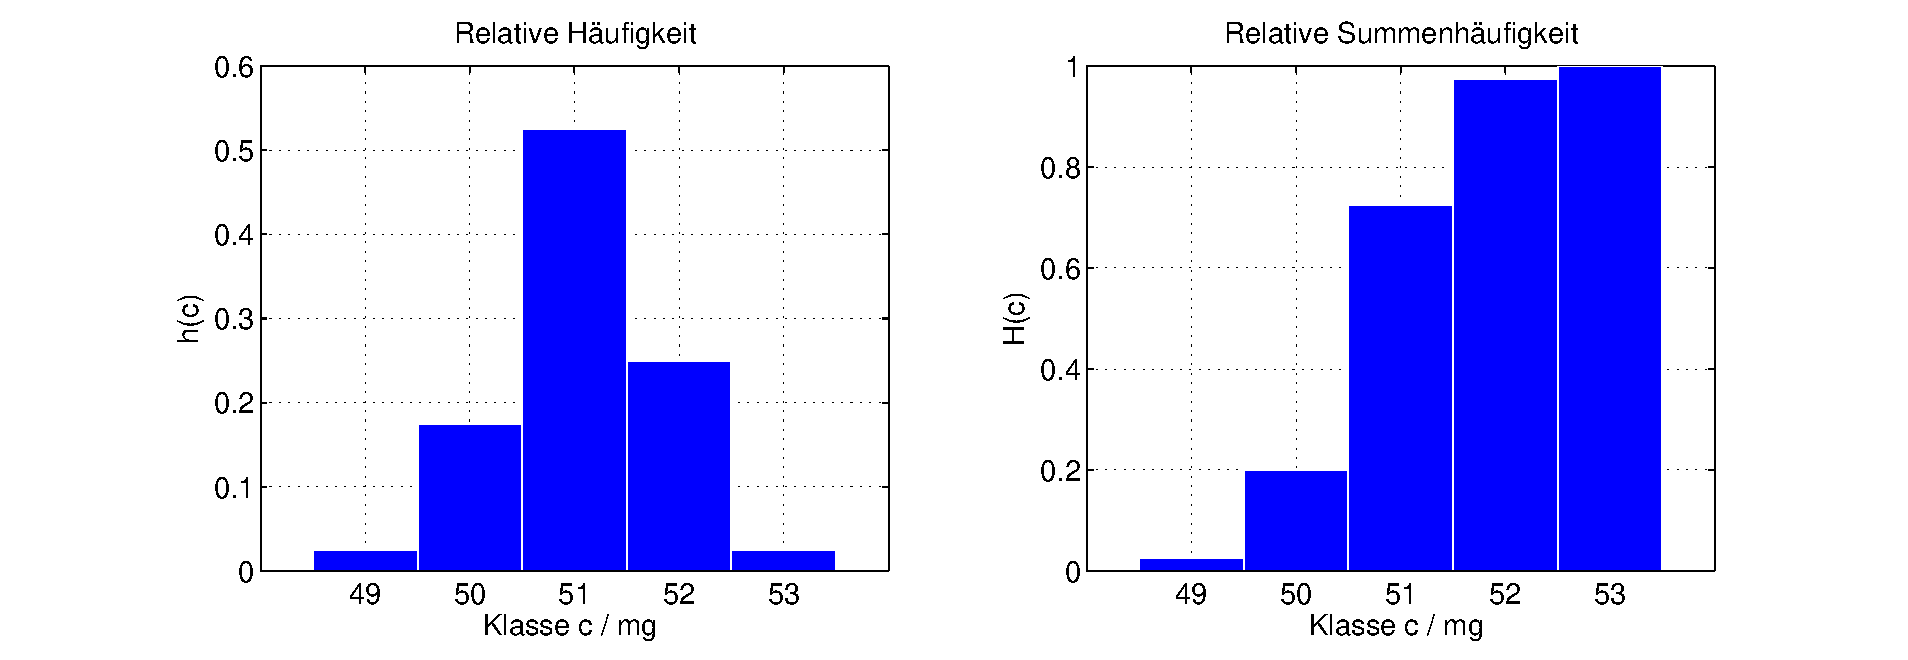
\includegraphics[width=1\textwidth]{Kapitel3/Bilder/image15}}
  \caption{Darstellung der relativen H\"{a}ufigkeit und der relativen Summenh\"{a}ufigkeit}
  \label{fig:DefinitionSchiefeBoxPlot2}
\end{figure}

\noindent Die Einteilung der Messwerte in Klassen erfolgt durch MATLAB. Die Berechnung der H\"{a}ufigkeiten und die Darstellung in Bild \ref{fig:DefinitionSchiefeBoxPlot2} werden mit der folgenden MATLAB-Befehlssequenz erstellt.

\lstinputlisting[caption = {}]{Kapitel3/mat4.m}

\noindent Zur numerischen Beschreibung der H\"{a}ufigkeitsverteilung werden analog zur Datenanalyse ohne Klasseneinteilung die Lage- und Streuungskennwerte berechnet. Hierbei muss die Klasseneinteilung der Messwerte ber\"{u}cksichtigt werden. Damit berechnet sich der arithmetische Mittelwert zu

\begin{equation}\label{eq:threeseventyfive}
\bar{m}=\displaystyle\sum _{n=1}^{N}\left(c_{n} \cdot h (c_{n})\right) =51.08 mg
\end{equation}

\noindent Der Median folgt nach den Darstellungen in Abschnitt 3.3.1 zu

\begin{equation}\label{eq:threeseventysix}
m_{MED} =c_{n-1} +\dfrac{d\cdot \left(0.5-H(c_{n-1} )\right)}{h\left(c_{n} \right)} =50 mg+\dfrac{1 mg\cdot (0.5-0.2)}{0.525} = 50.57 mg
\end{equation}

\noindent Die Berechnung der Streuungskennwerte f\"{u}hren zu einem Wert f\"{u}r die Varianz von

\begin{equation}\label{eq:threeseventyseven}
s^{2} =\dfrac{1}{N-1} \cdot \displaystyle\sum _{n=1}^{N}\left(h_{a} (c_{n})\cdot (c_{n} -\bar{m})^{2} \right) =6.19 mg^{2}
\end{equation}

\noindent und f\"{u}r die Standardabweichung von

\begin{equation}\label{eq:threeseventyeight}
s=\sqrt{s^{2} } =2.49 mg
\end{equation}

\noindent Der Interquartilabstand berechnet sich aus der Differenz aus dem 75\%-Quartil

\begin{equation}\label{eq:threeseventynine}
m_{0.75} =c_{n-1} +\dfrac{d\cdot \left(0.75-H\left(c_{n-1} \right)\right)}{h(c_{n})} =51 mg+\dfrac{1 mg\cdot (0.75-0.725)}{0.25} =51.10 mg
\end{equation}

\noindent und dem 25\%-Quartil

\begin{equation}\label{eq:threeeighty}
m_{0.25} =c_{n-1} +\dfrac{d\cdot \left(0.25-H(c_{n-1} )\right)}{h(c_{n})} =50 mg+\dfrac{1 mg\cdot \left(0.25-0.2\right)}{0.525} =50.0952 mg
\end{equation}

\noindent zu

\begin{equation}\label{eq:threeeightyone}
IQR=m_{0.75} -m_{0.25} =51.10 mg-50.0952 mg=1.00 mg
\end{equation}

\noindent Zur numerischen Auswertung der Daten wird die folgende Befehlssequenz verwendet.

\lstinputlisting[caption = {}]{Kapitel3/mat5.m}

\noindent Abschlie{\ss}end wird die Schiefe der H\"{a}ufigkeitsverteilung beurteilt. Bereits in Bild \ref{fig:DefinitionSchiefeBoxPlot2} ist ersichtlich, dass die Verteilung der relativen H\"{a}ufigkeit nahezu symmetrisch zu der Klasse von 51 mg ist. Es ist daher zu erwarten, dass sowohl der 25\%-Quartilkoeffizient als auch der Momentenkoeffizient der Schiefe einen Wert nahe 0 annehmen. Die Berechnung zeigt, dass sowohl der 25\%-Quartilkoeffizient der Schiefe mit

\begin{equation}\label{eq:threeeightytwo}
g_{0.25} =\dfrac{(m_{0.75} -m_{med})-(m_{med} -m_{0.25} )}{m_{0.75} -m_{0.25}}=\dfrac{(51.10-50.57)-(50.57-50.0952)}{51.10-50.0952} = 0.05
\end{equation}

\noindent als auch der Momentenkoeffizient der Schiefe mit

\begin{equation}\label{eq:threeeightythree}
g_{M} =\dfrac{\dfrac{1}{N} \cdot \sum _{n=1}^{N}(h_{a} (c_{n} )\cdot (c_{n} -\bar{m})^{3}) }{s^{3} } =-0.03
\end{equation}

\noindent diese Aussage bekr\"{a}ftigt. Die Berechnung mit MATLAB ergibt sich aus folgender Befehlssequenz.

\lstinputlisting[caption = {}]{Kapitel3/mat6.m}

\subsubsection{Vergleich der beiden Datenanalysen}

\noindent Die Daten aus Tabelle \ref{tab:threetwentythree} werden ohne eine Einteilung in Klassen und mit einer Einteilung in f\"{u}nf Klassen bewertet. Hierzu werden die eingef\"{u}hrten Lage- und Streuungskennwerte berechnet und die Gr\"{o}{\ss}en zur Bewertung der Schiefe bestimmt. Dabei weichen die Ergebnisse zwischen den beiden Analysemethoden voneinander ab. Um den Unterschied grafisch zu verdeutlichen, werden die Kennwerte der Datenanalyse mit und ohne eine Einteilung in Klassen als Box-Plot in \ref{fig:DefinitionSchiefeBoxPlot3} zusammengefasst und gegen\"{u}bergestellt.

\noindent 
\begin{figure}[H]
  \centerline{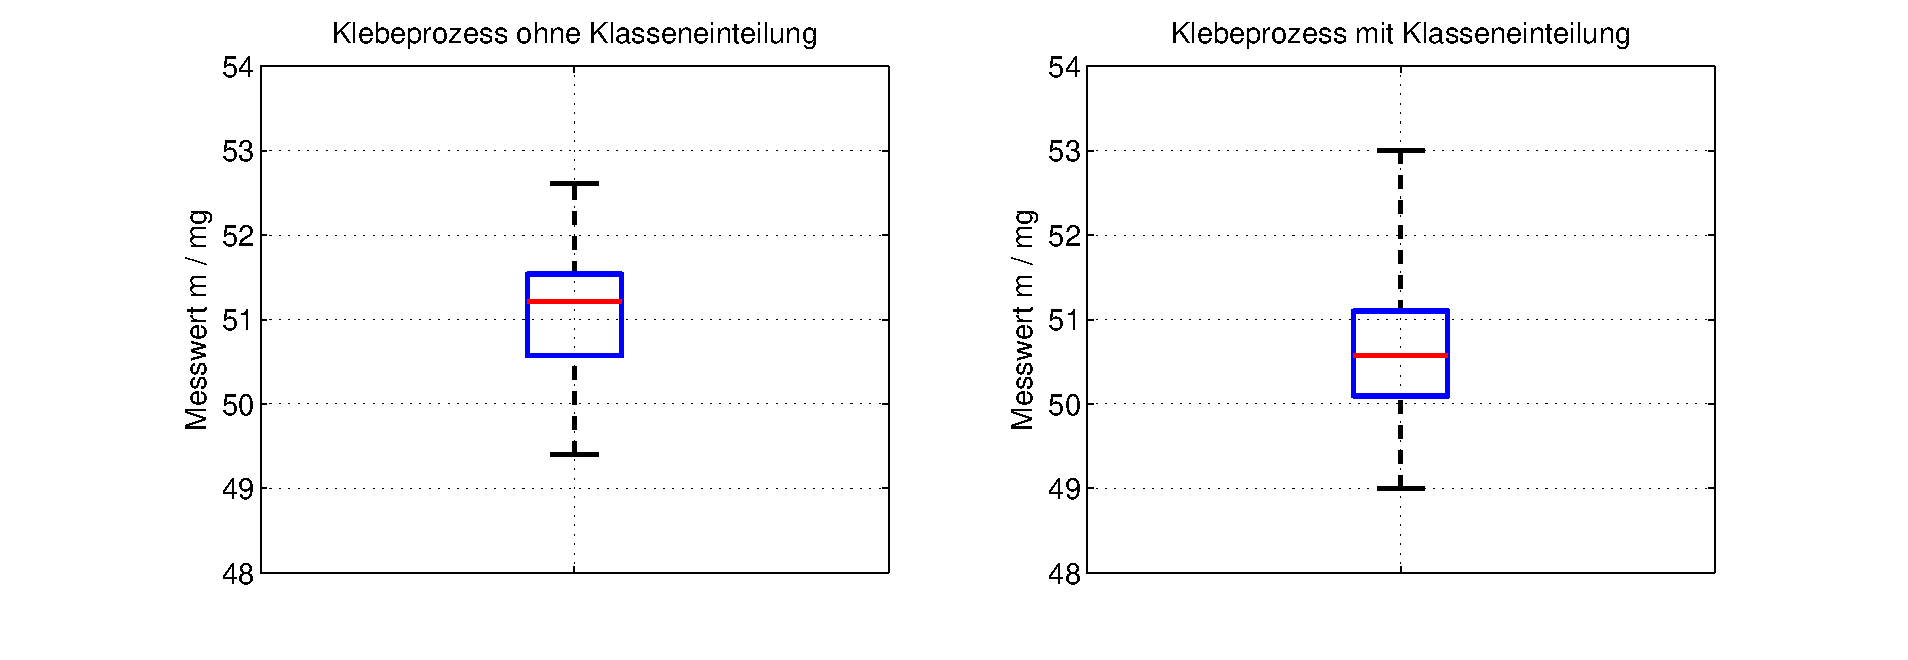
\includegraphics[width=1\textwidth]{Kapitel3/Bilder/image16}}
  \caption{Gegen\"{u}berstellung der beiden Datenanalysemethoden}
  \label{fig:DefinitionSchiefeBoxPlot3}
\end{figure}

\noindent Anhand des blauen Rechtecks in der Grafik des Box-Plots kann abgelesen werden, in welchem Bereich 50 \% der Stichprobenwerte liegen, die rote Linie kennzeichnet den Median der Verteilung. In \ref{fig:DefinitionSchiefeBoxPlot3} ist gut zu erkennen, dass die Auswertungen mit und ohne Klassenbildung stark voneinander abweichen. W\"{a}hrend der Median f\"{u}r den Klebeprozess ohne Klassenbildung bei m$_{MED}$ = 51.21 mg liegt, liegt er nach der Einteilung in Klassen bei m$_{MED}$ = 50.57 mg, der Wert differiert um 0.7 mg. Au{\ss}erdem ist zu erkennen, dass die Spannweite der Verteilung bei einer Betrachtung mit einer Einteilung in Klassen bei der vorliegenden Wahl der Klassenmitten gr\"{o}{\ss}er ist als bei einer Betrachtung ohne eine Einteilung in Klassen.\newline

\noindent Die unterschiedlichen Ergebnisse erkl\"{a}ren sich dadurch, dass mit der Klassenbildung die einzelnen Werte nicht mehr erfasst werden und dadurch Informationen \"{u}ber die Verteilung verloren gehen. Die Genauigkeit der Auswertung ist von der Klassenanzahl abh\"{a}ngig. Je weniger Klassen aus der Urliste gebildet werden, desto mehr Informationen gehen verloren und desto st\"{a}rker k\"{o}nnen die berechneten Kenngr\"{o}{\ss}en von den wahren Kenngr\"{o}{\ss}en der zu Grunde liegenden Verteilung abweichen. Aus diesem Grund sollte nach M\"{o}glichkeit stets mit der Urliste gearbeitet werden. \newline

\noindent Der verwendete Programmcode zur Darstellung des Box-Plots f\"{u}r die Messdaten ohne eine Einteilung in Klassen kann in MATLAB der folgenden Auflistung entnommen werden.

\lstinputlisting[caption = {}]{Kapitel3/mat7.m}

\noindent Der Box-Plot f\"{u}r die Zusammenfassung der Datenanalyse mit Einteilung in Klassen muss unter Verwendung der berechneten Kenngr\"{o}{\ss}en manuell programmiert werden, da MATLAB keine Funktionen zur Berechnung von Kenngr\"{o}{\ss}en gruppierter Daten zur Verf\"{u}gung stellt.

\subsubsection{Programmbeispiel zur Datenanalyse in Python}

\noindent Die Datenanalyse in Python erfordert zun\"{a}chste das Laden der erforderlichen Module und eine Definition des Ortes, an dem die Grafiken angezeigt werden sollen.

\lstinputlisting[caption = {}]{Kapitel3/mat8.m}

\noindent Die Daten liegen als mat-Datei vor. Python bietet einen Befehl zum Laden dieser Daten an. Die Daten werden in ein eindimensionales Array gewandelt.

\lstinputlisting[caption = {}]{Kapitel3/mat9.m}

\noindent Der Datenumfang und die statistischen Kennwerte werden mit den angegebenen Befehlen berechnet. Dabei werden die in MATLAB berechneten Ergebnisse best\"{a}tigt.

\lstinputlisting[caption = {}]{Kapitel3/mat10.m}

\noindent Die Daten werden mit einem Streudiagramm sowie einem Boxplot visualisiert.

\noindent 
\begin{figure}[H]
  \centerline{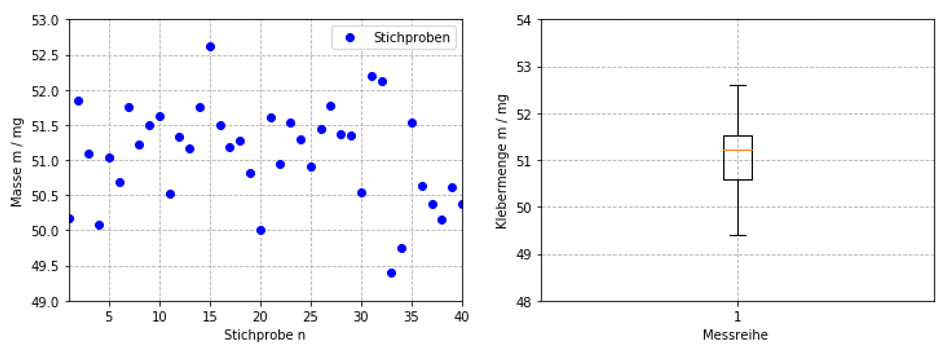
\includegraphics[width=1\textwidth]{Kapitel3/Bilder/image17}}
  \caption{Darstellung der Messwerte als Streudiagramm und Boxplot}
  \label{fig:Inconnue}
\end{figure}

\lstinputlisting[caption = {}]{Kapitel3/mat11.m}

\noindent Der steige Datensatz wird mit Hilfe von dem Modul Pandas in eine Tabelle gewandelt und ausgegeben. Dabei werden absolute und relative H\"{a}ufigkeit sowie die absolute und relative H\"{a}ufigkeit berechnet.

\clearpage

\lstinputlisting[caption = {}]{Kapitel3/mat12.m}

\noindent Das Ergebnis wird als Histogramm und mit seienr relativen Summenh\"{a}ufigkeit dargestellt.

\noindent 
\begin{figure}[H]
  \centerline{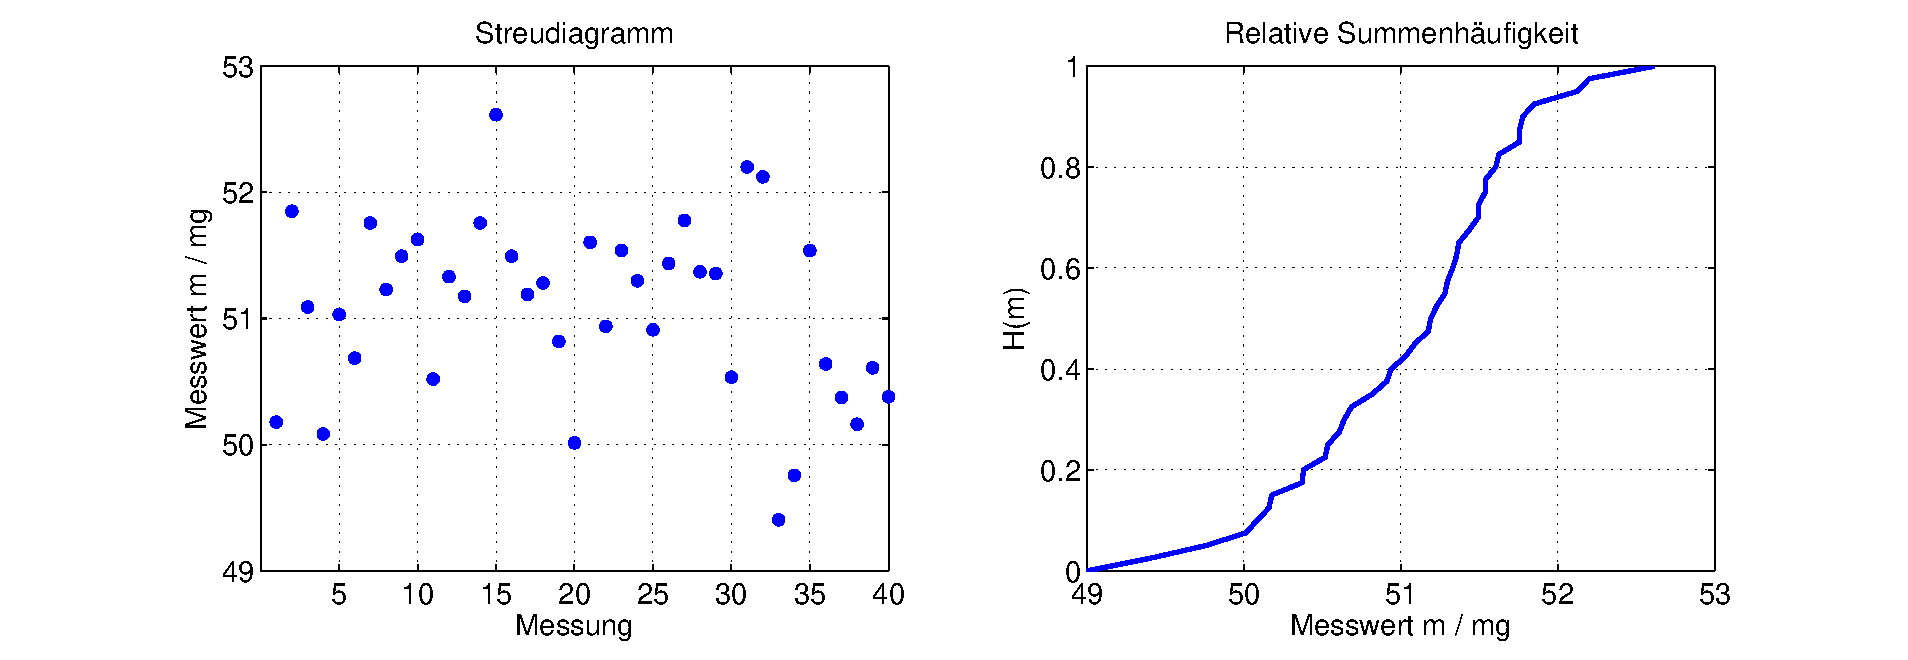
\includegraphics[width=1\textwidth]{Kapitel3/Bilder/image18}}
  \caption{Darstellung der Messwerte als Histogramm und relative Summenh\"{a}ufigkeit}
  \label{fig:AnwendungsbeispielKlebermenge1}
\end{figure}

\lstinputlisting[caption = {}]{Kapitel3/mat13.m}

\clearpage


\subsection{Literatur}

\begin{tabular}{|p{0.6in}|p{5.7in}|} \hline 
[Krey91] & Kreyszig, Erwin: Statistische Methoden und ihre Anwendungen\newline 
4., unver\"{a}nderter Nachdruck der 7. Auflage\newline 
Vandenhoeck \& Ruprecht, G\"{o}ttingen, 1991\\ \hline 
[Fahr06] & Fahrmeir, Ludwig; K\"{u}nstler, Rita; Pigeot, Iris; Tutz, Gerhard: Der Weg zur Datenanalyse\newline 
6. Auflage\newline 
Springer Berlin Heidelberg New York, 2006 \\ \hline 
[Ross06] & Ross, M. Sheldon: Statistik f\"{u}r Ingenieure und Naturwissenschaftler\newline 
3. Auflage\newline 
Spektrum Akademischer Verlag, M\"{u}nchen, 2006 \\ \hline 
\end{tabular}
